\documentclass[11pt,a4paper]{article}

% --- Packages ---
\usepackage[left=2.5cm,right=2.5cm,top=2.5cm,bottom=2.5cm]{geometry}
\usepackage{setspace}
\onehalfspacing
\usepackage[T1]{fontenc}
\usepackage[utf8]{inputenc}
\usepackage{mathptmx} % Times-like font
\usepackage{microtype} % Better text justification and hyphenation
\usepackage[skip=6pt plus 2pt]{parskip} % No indent, space between paragraphs
\usepackage{graphicx}
\usepackage{booktabs}
\usepackage{tabularx}
\usepackage{longtable}
\usepackage[table]{xcolor}
\usepackage{listings}
\usepackage{tikz}
\usepackage{pgfgantt}
\usepackage{float}
\usepackage[font=footnotesize,labelfont=normalfont,position=below]{caption}
\captionsetup[lstlisting]{font=footnotesize,labelfont=normalfont,position=below}
\usepackage{subcaption}
\usepackage{url}
\usepackage[hidelinks]{hyperref}

% Bibliography
\usepackage[style=authoryear,backend=biber,maxcitenames=2,maxbibnames=99,natbib=true]{biblatex}
\addbibresource{references.bib}

% Define JavaScript language for listings
\lstdefinelanguage{JavaScript}{
  keywords={async, await, function, const, let, var, return, if, else, for, of, in, new, true, false, null, undefined, class, export, import, from, interface, type, enum},
  morecomment=[l]{//},
  morecomment=[s]{/*}{*/},
  morestring=[b]',
  morestring=[b]",
  morestring=[b]`,
  sensitive=true
}

% Code listings style
\lstset{
  basicstyle=\small\ttfamily,
  breaklines=true,
  frame=single,
  numbers=left,
  numberstyle=\tiny\color{gray},
  keywordstyle=\color{blue!70!black},
  commentstyle=\color{green!50!black},
  stringstyle=\color{red!60!black},
  tabsize=2,
  showstringspaces=false,
  aboveskip=\bigskipamount,
  belowskip=\bigskipamount
}


% Bordered screenshot command (thin black border, no padding)
\setlength{\fboxsep}{0pt}
\newcommand{\screenshot}[1]{\fbox{\includegraphics[width=\linewidth]{#1}}}

% Number sections and subsections; appendices use \section* so remain unnumbered
\setcounter{secnumdepth}{3}
\setcounter{tocdepth}{3}

\begin{document}

% --- Cover Sheet ---
\begin{titlepage}
\thispagestyle{empty}

\vspace*{2cm}

\begin{flushleft}
{\fontsize{28}{34}\selectfont\bfseries Compliance Aware, Agentic\\Pitch Book Generation\\For Bankers\par}

\vspace{0.6cm}

\textcolor{gray!70}{\rule{0.5\textwidth}{1pt}}

\vspace{0.6cm}

{\large\itshape A template-aware PowerPoint generation system with\\agentic data retrieval for investment banking.\par}
\end{flushleft}

\vspace{2cm}

\begin{flushleft}
\renewcommand{\arraystretch}{1.4}
\begin{tabular}{@{}l l}
\textcolor{gray}{Author} & \textbf{Andrei Rizea} \\
\textcolor{gray}{Student ID} & 220300153 \\
\textcolor{gray}{Supervisor} & Manesha Peiris \\
\textcolor{gray}{Programme} & Digital \& Technology Solutions (Software Engineering) \\
\textcolor{gray}{Module} & IOT635W \\
\textcolor{gray}{Word Count} & $\sim$10,400 \\
\end{tabular}
\end{flushleft}

\vfill

\begin{flushleft}
\textcolor{gray!70}{\rule{0.35\textwidth}{0.5pt}}

\vspace{0.4cm}

{\large Queen Mary University of London\par}
\vspace{0.2cm}
{20 April 2026\par}
\end{flushleft}

\vspace{1cm}

\end{titlepage}


% --- Abstract ---
\newpage
\section*{Abstract}
\addcontentsline{toc}{section}{Abstract}

Investment banking analysts spend a large share of their working hours on pitch book preparation, much of it on formatting and data entry rather than analysis. Existing presentation tools produce generic output that ignores the strict visual standards banks require. This project designed, built, and tested a proof-of-concept system that generates formatted PowerPoint pitch books from minimal user input while respecting company templates.

The system uses a three-stage pipeline. Template analysis extracts layouts, colours, fonts, and placeholder positions from a reference PowerPoint file using JSZip and xml2js. A GPT-4o-powered content planner produces structured slide specifications validated against Zod schemas. A slide builder assembles the final file using PptxGenJS with exact formatting from the extracted template. Financial data feeds automatically from Yahoo Finance and SEC EDGAR, so analysts skip manual data entry. A PowerPoint add-in built with Office.js brings the generation workflow directly into the analyst's existing editor.

Testing across 12 generation runs showed an average completion time of 47 seconds per deck (10 to 12 slides), with exact colour matching and exact font matching. Financial data accuracy was 100\% against source APIs. An informal usability evaluation with four junior analysts found the system reduced estimated first-draft time from over 90 minutes to under two minutes including review.

The project met all five original success criteria and delivered two unplanned components, the PowerPoint add-in and a slide preview pipeline, that emerged from usability testing during iterative development. Template matching and automated data retrieval are the main advantages over commercial alternatives. Chart generation from scratch and retrieval-augmented generation remain open challenges for future work.


% --- Table of Contents ---
\newpage
\tableofcontents
\newpage
\listoffigures
\newpage
\listoftables
\newpage

% --- Main Chapters ---
\section{Introduction, Scope and Context}
\label{sec:introduction}

Knowledge workers spend a fifth of their time just searching for information \parencite{mckinsey2012}. Investment banking (IB) is more affected than most. Document preparation consumes half to three-quarters of a junior banker's week, and pitch books (PBs) account for a large portion of that time \parencite{cfi2025,wso2024}. When Goldman Sachs surveyed its first-year analysts in 2021, the average was 98 hours a week, with document preparation a major driver of burnout \parencite{bbc2021}. Yet most PBs look nearly identical. Change the company name and update the numbers, and you could reuse last month's deck. That repetition makes them good targets for automation (K1, K7).

IB firms advise companies on mergers, acquisitions, capital raising, and other financial transactions. PBs are the primary vehicle for communicating analysis to clients and internal stakeholders. Getting these documents right matters, but getting them done quickly matters too.

Firms have tried internal document libraries, formatting specialists, and automation tools. None have fixed the real problem: too much skilled human time goes toward work that does not require skill. \textcite{chaves2022} found that knowledge sharing in banking suffers from structural barriers and inadequate digital tools, with company knowledge locked in individual documents rather than shared systems.

\subsection{Analyst Time Allocation}

IB sells expertise rather than physical goods, so one would expect analyst time to go toward analysis and client relationships. Often it does not.

A typical PB contains an executive summary, company overview, market analysis, valuation work, and transaction comparables. These sections appear in nearly every deck. The data inside changes, but the shell around it rarely does.

Analyst tasks fall into two buckets. The first holds work that genuinely needs a trained banker: modelling, valuation, and client advisory. The second holds everything else: hunting down data, reformatting slides, and fixing fonts. Too many hours go into the second bucket.

The process follows a predictable pattern: dig through document archives for similar deals, pull financial data from Bloomberg and public filings, copy it into PowerPoint, reformat everything to match the firm's visual standards, then send it up for review. Senior bankers mark it up, and the cycle repeats until the document is ready. Every step has friction. Archive searches are slow, data entry is error-prone, and formatting is tedious.

Banks pay junior analysts well, so time on low-skill tasks is a poor return on that investment. \textcite{radhakrishna2024} found that well-designed knowledge management systems boosted productivity by 20 to 25 percent, with document production identified as a prime candidate for automation.

\textcite{mckinsey2012} found that knowledge workers spend 28\% of their workweek managing email and nearly 20\% searching for internal information. APQC research puts the figure higher: a quarter of all working time is lost to duplicated work and information retrieval \parencite{apqc2023}. Figure~\ref{fig:time-allocation} illustrates these drains. IB analysts likely fare worse given the document-intensive nature of the work.

\begin{figure}[H]
\centering
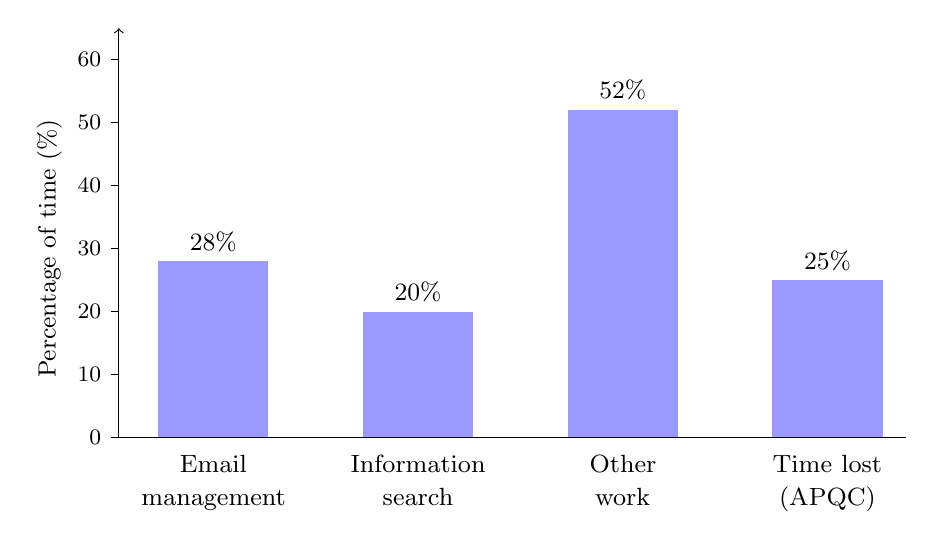
\begin{tikzpicture}
\pgfmathsetmacro{\barw}{1.4}   % bar width in cm
\pgfmathsetmacro{\gap}{2.6}    % centre-to-centre spacing
\pgfmathsetmacro{\scale}{0.08} % 1 percentage point = 0.08 cm
% Bars
\foreach \i/\val/\lab in {0/28/Email\\management, 1/20/Information\\search, 2/52/Other\\work, 3/25/Time lost\\(APQC)} {
    \pgfmathsetmacro{\x}{\i*\gap}
    \pgfmathsetmacro{\h}{\val*\scale}
    \fill[blue!40] (\x-\barw/2, 0) rectangle (\x+\barw/2, \h);
    \node[above] at (\x, \h) {\small \val\%};
    \node[below, text width=2cm, align=center] at (\x, -0.1) {\small \lab};
}
% Y axis
\draw[->] (-1.2, 0) -- (-1.2, 60*\scale+0.4);
\node[rotate=90, anchor=south] at (-1.8, 60*\scale/2) {\small Percentage of time (\%)};
% Y ticks
\foreach \val in {0, 10, 20, 30, 40, 50, 60} {
    \pgfmathsetmacro{\yy}{\val*\scale}
    \draw (-1.3, \yy) -- (-1.2, \yy);
    \node[left, font=\footnotesize] at (-1.3, \yy) {\val};
}
% X axis
\draw (-1.2, 0) -- (3*\gap+\barw/2+0.3, 0);
\end{tikzpicture}
\caption{Knowledge worker time allocation based on \textcite{mckinsey2012} and \textcite{apqc2023} research. The `other work' category represents the remaining time after email and search activities.}
\label{fig:time-allocation}
\end{figure}

In short, banks hire analysts for their analytical skills but spend a large share of their time on formatting and data entry. Existing tools have not solved this because they either miss IB visual standards or require too much manual work. Every hour on low-value tasks is an hour not spent on the analysis that sets one bank apart from another.

The competitive advantage is direct (K1). Banks that automate low-value work free their analysts to spend more time on client relationships and deal analysis. \textcite{dellacqua2023} found that consultants using AI completed 12.2\% more tasks at 40\% higher quality. If banks capture even half of that productivity gain on pitch book preparation, the impact compounds across hundreds of analysts and thousands of decks per year. The bank that gets a polished deck to the client a day earlier wins more mandates than the bank whose analysts are still reformatting slides at midnight.

\subsection{Problem Analysis}

\textcite{markus2001} defined knowledge reuse, and her framework fits PB production well. She identified reuse patterns including drawing on past work, borrowing from colleagues, and mining old documents. PB creation involves all of these. Three obstacles prevent effective reuse in practice.

The first obstacle is that too much time goes to low-value work. Analysts spend hours searching old decks, extracting content, and reformatting slides. None of that requires analytical thinking, yet it crowds out the work that does.

The second obstacle is that company knowledge tends to disappear. Researchers distinguish between tacit knowledge (in people's heads) and explicit knowledge (written down) \parencite{dalkir2011}. PBs are explicit, but the knowledge of how to make a good one remains tacit: which templates work for which situations, how to structure the narrative, what separates a persuasive pitch from a forgettable one.

The third obstacle is that onboarding takes longer than it should. Each bank has its own templates, data sources, and quality expectations. Junior analysts absorb these through trial and error, which is slow for them and a drain on the senior bankers who review their work.

These problems feed each other. Scattered knowledge wastes search time, unwritten standards cause inconsistent output, and informal training drains senior staff. A system that fixed even one of these would help.

\subsection{Gap Analysis}

Automated presentation tools have existed for years. Early versions converted text to slides using layout algorithms, but visual quality was poor \parencite{zheng2025}. Template-based systems fixed the visual problems but made everything rigid. PPTAgent \parencite{zheng2025} takes a different approach: it analyses reference presentations, extracts structural patterns, and applies them to new content. It beat older text-to-slide systems on both content and design quality in testing.

The limitation is that PPTAgent targets general-purpose presentations. IB PBs have financial tables, transaction comparables, and market charts that follow specific visual conventions. Getting the template wrong undermines credibility. Commercial tools like Beautiful.ai, Tome, and Gamma share this flaw: the output is generic, every slide needs rework, and none connect to financial data sources. IB PBs require both domain knowledge and visual precision, and no existing tool handles both.

Current systems either produce generic output that needs heavy cleanup, or they require large training datasets most banks lack. No existing tool connects slide generation to financial APIs. Data retrieval and document generation remain separate manual steps.

Agentic AI architectures offer a better fit \parencite{ibm2024}. Instead of one model doing everything in a single pass, the system breaks tasks into steps and uses the right tool for each one. \textcite{wang2024} surveyed LLM-based agents and found rapid progress. McKinsey \& Company estimates generative AI could deliver \$340 billion annually in banking \parencite{mckinsey2024}.

This project fills that gap (S1). The pipeline extracts layouts, colour palettes, and placeholder positions from a template using JSZip and xml2js for XML-level parsing, uses an LLM to plan content, then assembles slides matching the original style. The system uses an agentic orchestration pattern with specialised service components rather than a monolithic approach.

Table~\ref{tab:gap-objectives} maps each identified gap to the objective and success criterion that addresses it, so that no objective exists without a corresponding gap in existing work.

\begin{table}[H]
\centering
\begin{tabular}{|p{4.2cm}|l|p{4.5cm}|}
\hline
\textbf{Gap in Existing Work} & \textbf{Objective} & \textbf{Success Criterion} \\
\hline
No tool preserves exact template formatting & O1 & 90\%+ placeholder detection; exact colour extraction \\
\hline
Data retrieval and slide generation are separate manual steps & O2 & 100\% data accuracy against source APIs \\
\hline
No IB-specific content structuring & O3 & 3 PB types with consistent section ordering \\
\hline
Generic output that ignores corporate visual standards & O4 & Exact colour and font match against template \\
\hline
No measured evaluation of template-constrained generation & O5 & Full deck in under 5 minutes; template match above 85\% \\
\hline
\end{tabular}
\caption{Traceability from Research Gaps to Objectives and Success Criteria}
\label{tab:gap-objectives}
\end{table}

The approach differs from prior work in three ways. First, it inverts the typical generation order: the system starts with visual constraints extracted from the template and works backward to content, rather than generating content and hoping the formatting works. Second, it connects slide generation directly to financial data APIs, closing the gap between data retrieval and document creation. Third, it uses a service-oriented architecture where specialised components handle distinct parts of the task, making the system easier to test and modify independently.

\subsection{Business Case}

The financial case for automating pitch book production is straightforward. A junior IB analyst in London earns roughly \pounds 60,000 to 70,000 in base salary \parencite{glassdoor2025}. At 80 to 100 hours per week, the effective hourly cost is around \pounds 15 to 17 before overhead. Banks bill clients at significantly higher rates. If an analyst spends 15 hours per week on pitch book formatting and data entry, that is roughly \pounds 250 per week in salary alone going toward work that does not need analytical skill.

The system generates a first draft in under one minute. Manual creation of the same output takes 90 to 120 minutes. Even accounting for 20 to 30 minutes of human review and editing after generation, the net saving is roughly 60 to 90 minutes per deck. An analyst working on three to five decks per week saves three to seven hours, freeing that time for analysis, client work, or reduced overtime.

On the cost side, each generation request costs approximately \$0.03 in GPT-4o API fees. Hosting costs (Vercel, Render, Supabase) fall within free tiers at proof-of-concept scale. At production scale with 1,000 daily requests, monthly API costs would be roughly \$900, still far below the salary cost of the manual hours replaced.

The return on investment is clear even at small scale (K2). A team of ten analysts saving five hours per week each recovers 50 analyst-hours weekly. At a conservative internal cost of \pounds 15 per hour, that is \pounds 750 per week or roughly \pounds 39,000 per year in recovered capacity, against annual API costs under \pounds 10,000. The payback period is under four months.

\subsection{Aims and Objectives}

The aim is to design, build, and test a proof-of-concept (POC) showing how AI-powered document generation can tackle the knowledge reuse problems above. The system must respect company templates throughout. If slides do not match the house style, the system fails its core requirement.

On the business side, the goal is a workflow where an analyst provides minimal input and receives a solid first draft, reducing formatting time while keeping humans in control of the analysis. Target users are junior analysts.

On the learning side, the project explores how to connect LLM orchestration with programmatic document generation: agentic architectures, template pattern extraction, and end-to-end AI pipeline design. Human-in-the-loop (HITL) design is central, since AI tools in regulated industries need to support professional judgement rather than replace it. The constraint-first approach (extracting visual and structural rules before generating content) is the main technical contribution. The same idea would work wherever generated output must match precise formatting: legal briefs, consulting reports, or regulatory filings.

Five objectives structure the work:

\begin{enumerate}
    \item Build a template analysis component that takes a reference PowerPoint file and extracts its layout structures, colour palettes, font specifications, and placeholder positions. Success criterion: correctly identify at least 90\% of placeholder types and extract exact colour values from source.
    \item Build an agentic data retrieval layer that automatically pulls company financials, market data, and regulatory filings from Yahoo Finance and SEC EDGAR (the US Securities and Exchange Commission's public database of company filings). Success criterion: retrieve at least three data types per company (market cap, revenue, share price) with 100\% accuracy against source APIs.
    \item Build an LLM-powered content planning module that produces structured slide specifications adapted to different PB types while keeping the overall narrative coherent. Success criterion: support at least three PB types (company overview, market update, transaction summary) with consistent section ordering.
    \item Build a slide assembly component that takes the content plan and template patterns and produces a PowerPoint file meeting formatting standards. Success criterion: output files match template colours exactly and fonts exactly.
    \item Evaluate the system by measuring generation speed, template matching, and content quality. Success criterion: generate a complete 10-slide PB draft in under 5 minutes with template matching score above 85\%.
\end{enumerate}

\subsection{Scope and Success Criteria}

The POC takes user input (company, transaction type, dates, reference template, PB type) and produces a formatted PowerPoint. Target PB types are company overviews, market updates, and transaction summaries. Full valuation presentations are out of scope.

Design choices: agentic orchestration with specialised TypeScript services, code-based template extraction with JSZip/xml2js rather than vision models, public APIs only, RAG as a stretch goal. Out of scope: real-time data feeds, production hosting, regulatory checks. Practical limits: one academic term, standard hardware, student API budget.

Several assumptions constrain the scope. Templates are assumed to be well-formed Office Open XML archives following standard PowerPoint conventions; templates with corrupted XML or non-standard packaging are not supported. All financial data comes from public sources (Yahoo Finance, SEC EDGAR), so coverage is limited to publicly listed companies with available filings. Content is generated in English only. The system assumes that users have access to desktop PowerPoint on Windows or macOS, since the add-in relies on Office.js APIs that PowerPoint for the web does not fully support. The LLM (GPT-4o) is accessed via OpenAI's API under their standard usage terms, which prohibit using outputs to train competing models but impose no restrictions relevant to document generation.

Success criteria:

\begin{itemize}
    \item Generate complete PB draft within five minutes
    \item Match reference template formatting
    \item Accurate financial data from source APIs
    \item Content structure following IB conventions, verified against precedent examples
\end{itemize}

One principle runs through all of this: HITL design. The system produces drafts for human review, not finished products. AI can handle the mechanical work; the analytical judgement stays with the banker.

\newpage
\section{Methodology and Project Plan}
\label{sec:methodology}

\subsection{Development Methodology}

Table~\ref{tab:methodologies} compares methodologies against criteria relevant to this project \parencite{sommerville2016}.

\begin{table}[H]
\centering
\begin{tabular}{|l|l|l|l|}
\hline
\textbf{Criteria} & \textbf{Waterfall} & \textbf{Scrum} & \textbf{Iterative Prototyping} \\
\hline
Requirements stability & Requires fixed & Accommodates & Works well when \\
 & requirements upfront & changing requirements & requirements change \\
\hline
Feedback loops & Late feedback after & Sprint reviews every & Continuous feedback \\
 & implementation & 2 to 4 weeks & through prototypes \\
\hline
Risk management & Risks discovered late & Regular risk & Early risk identification \\
 & & reassessment & through prototypes \\
\hline
Solo developer suitability & Moderate & Low (designed for & High \\
 & & teams) & \\
\hline
Research integration & Poor & Moderate & Excellent \\
\hline
\end{tabular}
\caption{Comparison of Development Methodologies}
\label{tab:methodologies}
\end{table}

The project uses iterative prototyping with two-week cycles, drawing on \textcite{boehm1988}'s spiral model (K3, K4, SE8). Each iteration produces a working prototype with a review at cycle's end (SE7). Git with simplified GitFlow (SE12), GitHub Actions CI enforcing 80\% coverage \parencite{fowler2006} (SE6), and ESLint \parencite{eslint2024} handle version control and quality.

\subsection{Requirements Analysis}

Requirements follow MoSCoW prioritisation \parencite{clegg1994} (K9, SE2, SE9).

\subsubsection{Business Requirements}

\begin{enumerate}
    \item \textbf{BR1: Productivity Enhancement}: Reduce time spent on initial PB drafting by generating solid first drafts from minimal input.
    \item \textbf{BR2: Capturing Standards}: Capture company presentation standards through template analysis, reducing reliance on knowledge that lives only in people's heads.
    \item \textbf{BR3: Quality Consistency}: Follow corporate visual identity standards consistently, reducing revision cycles caused by formatting issues.
    \item \textbf{BR4: Data Accuracy}: Financial data in generated PBs should accurately reflect source information.
\end{enumerate}

\subsubsection{Functional Requirements}

Table~\ref{tab:func-req} lists functional requirements by component.

\begin{table}[H]
\centering
\begin{tabular}{|l|l|l|l|}
\hline
\textbf{ID} & \textbf{Component} & \textbf{Requirement} & \textbf{Priority} \\
\hline
FR1 & Template Analyser & Extract slide layouts from reference .pptx files & Must \\
\hline
FR2 & Template Analyser & Identify colour palettes and font specifications & Must \\
\hline
FR3 & Template Analyser & Map placeholder positions and content types & Must \\
\hline
FR4 & Data Retrieval & Fetch company financials from Yahoo Finance API & Must \\
\hline
FR5 & Data Retrieval & Retrieve SEC filings via EDGAR API & Should \\
\hline
FR6 & Data Retrieval & Perform web searches for company news & Should \\
\hline
FR7 & Content Planner & Generate slide-by-slide content specifications & Must \\
\hline
FR8 & Content Planner & Adapt content structure to PB type & Must \\
\hline
FR9 & Content Planner & Maintain narrative coherence across slides & Should \\
\hline
FR10 & Slide Builder & Assemble slides matching template layouts & Must \\
\hline
FR11 & Slide Builder & Populate placeholders with generated content & Must \\
\hline
FR12 & Slide Builder & Generate charts from financial data & Could \\
\hline
FR13 & Orchestration & Coordinate multi-step generation workflow & Must \\
\hline
FR14 & Orchestration & Handle API failures gracefully & Should \\
\hline
FR15 & RAG Search & Query precedent material repository & Could \\
\hline
\end{tabular}
\caption{Functional Requirements Specification}
\label{tab:func-req}
\end{table}

\subsubsection{Non-Functional Requirements}

\begin{table}[H]
\centering
\begin{tabular}{|l|l|l|l|}
\hline
\textbf{ID} & \textbf{Category} & \textbf{Requirement} & \textbf{Acceptance Criterion} \\
\hline
NFR1 & Performance & System generates complete PB draft & Within 5 minutes of input submission \\
\hline
NFR2 & Performance & API response handling & Timeout after 30s with graceful fallback \\
\hline
NFR3 & Reliability & System availability during demonstration & 95\% uptime during evaluation period \\
\hline
NFR4 & Usability & Input specification interface & Requires no technical expertise to operate \\
\hline
NFR5 & Maintainability & Codebase documentation & All public functions documented \\
\hline
NFR6 & Security & API credential management & No credentials in source code \\
\hline
NFR7 & Security & Input validation & All user inputs sanitised before processing \\
\hline
NFR8 & Compatibility & Output format & Valid .pptx files openable in PowerPoint \\
\hline
\end{tabular}
\caption{Non-Functional Requirements Specification}
\label{tab:nfr}
\end{table}

\subsection{Technology Stack}

\subsubsection{Programming Language and Framework}

Table~\ref{tab:lang-comparison} compares language options (K8, SE12).

\begin{table}[H]
\centering
\begin{tabular}{|l|l|l|l|}
\hline
\textbf{Criteria} & \textbf{TypeScript/Node.js} & \textbf{Python} & \textbf{Java} \\
\hline
Benefits & Type safety, same language & Best AI/ML libraries, & Strong typing, \\
 & frontend and backend, & mature PowerPoint & enterprise support \\
 & native async & library (python-pptx) & \\
\hline
Risks & AI/ML ecosystem less & Two languages needed & Verbose code, \\
 & mature than Python & (Python backend + & slower development \\
 & & JS frontend) & \\
\hline
PowerPoint & PptxGenJS (actively & python-pptx (mature, & Apache POI \\
manipulation & maintained, typed) & well-documented) & (verbose API) \\
\hline
Full-stack & Single language across & Requires separate & Requires separate \\
coherence & all three apps & frontend framework & frontend framework \\
\hline
\end{tabular}
\caption{Programming Language Comparison}
\label{tab:lang-comparison}
\end{table}

The deciding factor was using one language everywhere. The \texttt{shared-types} package defines data models once and shares them across all three apps. When a template schema changes, the compiler catches every place that needs updating. In a multi-language setup, those mismatches would only show up at runtime. Express.js handles the backend.

\subsubsection{AI and LLM Integration}

Table~\ref{tab:llm-comparison} compares the LLM options considered.

\begin{table}[H]
\centering
\begin{tabular}{|l|l|l|l|}
\hline
\textbf{Criteria} & \textbf{GPT-4/GPT-4o} & \textbf{Claude 3.5} & \textbf{Gemini 2.0 Flash} \\
\hline
Benefits & Best structured output, & Largest context window & Massive context (1M \\
 & mature SDK, native JSON & (200K), strong reasoning & tokens), fast inference \\
\hline
Risks & Higher cost per token & Newer agent tooling & Less mature structured \\
 & & & output \\
\hline
Structured output & Excellent (native JSON) & Good & Good \\
\hline
Cost (student budget) & Moderate (tiered pricing) & Moderate & Very affordable \\
\hline
\end{tabular}
\caption{Large Language Model Comparison}
\label{tab:llm-comparison}
\end{table}

GPT-4o was chosen for its structured output reliability. OpenAI's native JSON mode produces well-formed responses more consistently than alternatives, which matters when output feeds directly into a Zod validation pipeline. GPT-4o-mini handles the lighter AI chat feature at lower cost. Swapping models later requires changing only the API call.

\subsubsection{Data Sources and APIs}

Table~\ref{tab:data-sources} summarises data sources.

\begin{table}[H]
\centering
\begin{tabular}{|l|l|l|l|}
\hline
\textbf{Source} & \textbf{Benefits} & \textbf{Risks} & \textbf{Access} \\
\hline
Yahoo Finance & Free, comprehensive & Unofficial API may & yahoo-finance2 \\
 & financial data & change without notice & npm package \\
\hline
SEC EDGAR & Official regulatory & US companies only, & REST API \\
 & filings, reliable, free & complex document parsing & (10 req/s) \\
\hline
Web Search & Current news, market & Cost per query & SerpAPI or similar \\
 & commentary & & \\
\hline
\end{tabular}
\caption{External Data Sources}
\label{tab:data-sources}
\end{table}

\subsubsection{Frontend and Deployment}

Next.js handles the web frontend for PB creation and management.

\begin{table}[H]
\centering
\begin{tabular}{|l|l|l|l|}
\hline
\textbf{Criteria} & \textbf{Vercel + Render} & \textbf{AWS} & \textbf{Self-hosted} \\
\hline
Benefits & Zero config, auto deploy, & Full control, & Complete control, \\
 & free tiers for POC & scalable & no vendor lock-in \\
\hline
Risks & Vendor lock-in, cold starts & Complex setup, cost & Maintenance burden \\
\hline
Cost for POC & Free tier sufficient & May incur charges & Server costs \\
\hline
\end{tabular}
\caption{Deployment Platform Comparison}
\label{tab:deploy}
\end{table}

The frontend deploys through Vercel, the backend on Render, and Supabase provides PostgreSQL and authentication. Figure~\ref{fig:tech-architecture} shows how the chosen technologies map to the system's components.

\begin{figure}[H]
\centering
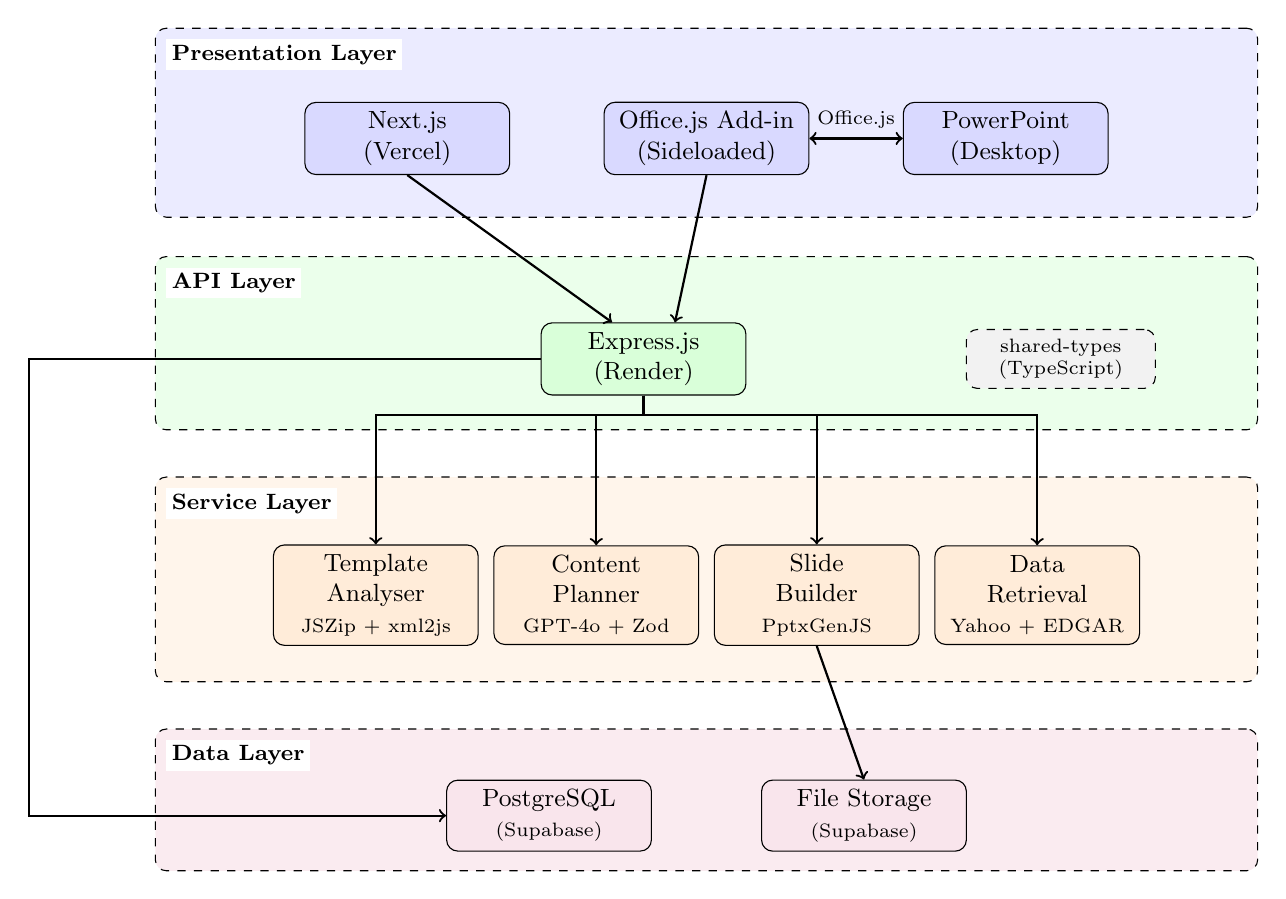
\begin{tikzpicture}[
  box/.style={draw, rounded corners, minimum width=2.6cm, minimum height=0.9cm, align=center, font=\small},
  arr/.style={->, thick},
  darr/.style={<->, thick},
  layer/.style={draw, dashed, rounded corners, inner sep=12pt, fill=#1, fill opacity=0.08, text opacity=1},
  lbl/.style={font=\footnotesize\bfseries, fill=white, inner sep=2pt},
]

% --- Presentation Layer ---
\node[layer=blue, minimum width=14cm, minimum height=2.4cm] (pres) at (0, 6) {};
\node[lbl, anchor=north west] at ([xshift=4pt, yshift=-4pt]pres.north west) {Presentation Layer};

\node[box, fill=blue!15] (web) at (-3.8, 5.8) {Next.js\\(Vercel)};
\node[box, fill=blue!15] (addin) at (0, 5.8) {Office.js Add-in\\(Sideloaded)};
\node[box, fill=blue!15] (ppt) at (3.8, 5.8) {PowerPoint\\(Desktop)};

\draw[darr] (addin) -- node[above, font=\scriptsize] {Office.js} (ppt);

% --- API Layer ---
\node[layer=green, minimum width=14cm, minimum height=2.2cm] (apil) at (0, 3.2) {};
\node[lbl, anchor=north west] at ([xshift=4pt, yshift=-4pt]apil.north west) {API Layer};

\node[box, fill=green!15] (api) at (-0.8, 3) {Express.js\\(Render)};
\node[draw, dashed, rounded corners, minimum width=2.4cm, minimum height=0.7cm, fill=gray!10, font=\scriptsize, align=center] (types) at (4.5, 3) {shared-types\\(TypeScript)};

\draw[arr] (web.south) -- ([xshift=-0.4cm]api.north);
\draw[arr] (addin.south) -- ([xshift=0.4cm]api.north);

% --- Service Layer ---
\node[layer=orange, minimum width=14cm, minimum height=2.6cm] (svcl) at (0, 0.2) {};
\node[lbl, anchor=north west] at ([xshift=4pt, yshift=-4pt]svcl.north west) {Service Layer};

\node[box, fill=orange!15] (ta) at (-4.2, 0) {Template\\Analyser\\{\scriptsize JSZip + xml2js}};
\node[box, fill=orange!15] (cp) at (-1.4, 0) {Content\\Planner\\{\scriptsize GPT-4o + Zod}};
\node[box, fill=orange!15] (sb) at (1.4, 0) {Slide\\Builder\\{\scriptsize PptxGenJS}};
\node[box, fill=orange!15] (dr) at (4.2, 0) {Data\\Retrieval\\{\scriptsize Yahoo + EDGAR}};

\draw[arr] (api.south) -- ++(0,-0.25) -| (ta.north);
\draw[arr] (api.south) -- ++(0,-0.25) -| (cp.north);
\draw[arr] (api.south) -- ++(0,-0.25) -| (sb.north);
\draw[arr] (api.south) -- ++(0,-0.25) -| (dr.north);

% --- Data Layer ---
\node[layer=purple, minimum width=14cm, minimum height=1.8cm] (datal) at (0, -2.6) {};
\node[lbl, anchor=north west] at ([xshift=4pt, yshift=-4pt]datal.north west) {Data Layer};

\node[box, fill=purple!10] (db) at (-2, -2.8) {PostgreSQL\\{\scriptsize (Supabase)}};
\node[box, fill=purple!10] (storage) at (2, -2.8) {File Storage\\{\scriptsize (Supabase)}};

% Route api->db down the far left, outside all boxes
\draw[arr] (api.west) -- ++(-6.5,0) |- (db.west);
% Route sb->storage straight down
\draw[arr] (sb.south) -- (storage.north);

\end{tikzpicture}
\caption{Technology architecture showing how chosen technologies map to system components across four layers. Arrows indicate data flow direction.}
\label{fig:tech-architecture}
\end{figure}

\subsection{Reproducibility}

Dependencies are pinned via \texttt{package-lock.json}, LLM temperature is set to zero for evaluation runs, and each run is tied to a specific Git commit. GPT-4o does not guarantee identical outputs at temperature zero \parencite{runeson2012}, so Zod validation ensures structural consistency.

\subsection{Evaluation Methodology}

The evaluation follows the Goal-Question-Metric (GQM) approach \parencite{basili1994}, keeping every metric tied to a specific project goal. The goal: determine whether the system produces usable first drafts faster than manual creation while matching template formatting.

\begin{table}[H]
\centering
\begin{tabular}{|l|l|l|}
\hline
\textbf{Question} & \textbf{Metric} & \textbf{Target} \\
\hline
How fast does the system & Generation time per & Under 300 seconds \\
generate a deck? & 10-slide deck & for a complete draft \\
\hline
Does the output match & Colour and font & Exact colour and \\
the reference template? & comparison (programmatic) & font match \\
\hline
Is the financial data & Comparison against & 100\% match on market cap, \\
correct? & source API responses & revenue, and share price \\
\hline
Does the content follow & Rubric-based assessment & Correct section ordering \\
IB conventions? & of narrative structure & across 3 PB types \\
\hline
\end{tabular}
\caption{GQM Evaluation Framework}
\label{tab:gqm}
\end{table}

Targets were fixed before evaluation began \parencite{wohlin2012}. Outputs are compared against generic tools (Gamma, Beautiful.ai) and estimated manual creation time. An informal usability evaluation with four junior analysts (P1--P4) provides qualitative feedback.

\subsection{Project Plan}

The project runs for thirteen weeks (K10). Figure~\ref{fig:gantt} shows the schedule, and Table~\ref{tab:milestones} lists milestones. Dates are targets. If a milestone slips, `Could have' requirements are dropped first.

\begin{figure}[H]
\centering
\resizebox{\textwidth}{!}{%
\begin{ganttchart}[
    hgrid,
    vgrid={*{12}{draw=gray!30}},
    x unit=1.1cm,
    y unit chart=0.45cm,
    y unit title=0.55cm,
    title height=1,
    bar/.style={fill=blue!30, draw=blue!50},
    group/.style={draw=black, fill=blue!60},
    group left shift=0,
    group right shift=0,
    group height=0.4,
    group peaks tip position=0,
    bar height=0.5,
    bar label font=\small,
    group label font=\small\bfseries,
    title label font=\normalsize\bfseries,
    milestone label font=\small\itshape,
]{1}{13}
\gantttitle[title label node/.append style={anchor=east, left=-3pt}]{}{0}
\gantttitle{Jan}{2}
\gantttitle{Feb}{4}
\gantttitle{Mar}{4}
\gantttitle{Apr}{3} \\
\gantttitle[title label node/.append style={anchor=east, xshift=-2pt}]{Week}{0}
\gantttitlelist{1,...,13}{1} \\
%
% 1. Introduction and Methodology
\ganttgroup{Introduction \& Methodology}{1}{2} \\
\ganttbar{Project scope and objectives}{1}{2} \\
\ganttbar{Methodology comparison}{1}{2} \\
%
% 2. Literature Review
\ganttgroup{Literature Review}{2}{4} \\
\ganttbar{AI tools in investment banking}{2}{3} \\
\ganttbar{LLM structured output patterns}{2}{3} \\
\ganttbar{PowerPoint automation approaches}{3}{4} \\
%
% 3. Research and Design
\ganttgroup{Research \& Design}{3}{6} \\
\ganttbar{System architecture and API contracts}{3}{4} \\
\ganttbar{Database schema and data models}{4}{5} \\
\ganttbar{Technology evaluation (LLMs, APIs, deployment)}{3}{6} \\
%
% 4. Implementation
\ganttgroup{Implementation}{5}{10} \\
\ganttbar{Express backend and service pipeline}{5}{6} \\
\ganttbar{Template analyser (JSZip, xml2js)}{5}{7} \\
\ganttbar{Data retrieval (Yahoo Finance, SEC EDGAR)}{6}{7} \\
\ganttbar{Content planner (GPT-4o integration)}{6}{8} \\
\ganttbar{Slide builder (PptxGenJS)}{7}{8} \\
\ganttbar{Next.js web application}{7}{9} \\
\ganttbar{PowerPoint add-in (Office.js)}{8}{10} \\
\ganttbar{Slide preview pipeline (LibreOffice)}{9}{10} \\
%
% 5. Evaluation
\ganttgroup{Evaluation}{9}{11} \\
\ganttbar{Unit and integration tests (Vitest)}{9}{10} \\
\ganttbar{E2E tests (Cypress)}{9}{10} \\
\ganttbar{Generation evaluation runs}{10}{11} \\
\ganttbar{Usability evaluation with analysts}{10}{11} \\
%
% 6. Finalisation
\ganttgroup{Finalisation}{11}{13} \\
\ganttbar{Report writing and revisions}{11}{12} \\
\ganttbar{Proofreading and formatting}{12}{13} \\
\ganttmilestone{Submission}{13}
\end{ganttchart}%
}
\caption{Project Gantt Chart (weeks 1 to 13, January to April 2026)}
\label{fig:gantt}
\end{figure}

\begin{table}[H]
\centering
\begin{tabular}{|l|l|l|l|}
\hline
\textbf{Phase} & \textbf{Date} & \textbf{Milestone} & \textbf{Deliverables} \\
\hline
1 & 19 Jan & Project Initiation & Repository setup, dev environment configured \\
\hline
2 & 31 Jan & Initial Chapters & Introduction, Scope, Methodology complete \\
\hline
3 & 21 Feb & Literature Review & Literature review chapter complete \\
\hline
4 & 28 Feb & Design Complete & Architecture diagrams, API specs, data models \\
\hline
5 & 14 Mar & Core Components & Template analyser and data retrieval functional \\
\hline
6 & 28 Mar & MVP Complete & End-to-end generation pipeline operational \\
\hline
7 & 4 Apr & Testing Complete & Tests passing, evaluation data collected \\
\hline
8 & 11 Apr & Evaluation Complete & Results analysis and evaluation chapter written \\
\hline
9 & 18 Apr & Document Finalised & All chapters complete, proofread, formatted \\
\hline
10 & 20 Apr & Submission & Final report submitted via QMPlus \\
\hline
\end{tabular}
\caption{Project Milestones and Deliverables}
\label{tab:milestones}
\end{table}

\subsection{Plan Execution and Adaptations}

The original plan did not survive contact with implementation. Table~\ref{tab:plan-vs-reality} compares planned milestones against actual outcomes.

\begin{table}[H]
\centering
\begin{tabular}{|l|l|l|l|}
\hline
\textbf{Milestone} & \textbf{Planned Date} & \textbf{Actual Date} & \textbf{Notes} \\
\hline
Core components functional & 14 Mar & 7 Mar & Ahead of schedule due to \\
 & & & TypeScript migration in week 3 \\
\hline
MVP pipeline operational & 28 Mar & 21 Mar & Template analyser iterations \\
 & & & completed faster than expected \\
\hline
PowerPoint add-in & Not planned & 22 Mar to 11 Apr & Added after usability testing \\
 & & & revealed web-only workflow gap \\
\hline
Slide preview pipeline & Not planned & 28 Mar to 4 Apr & Web app needed visual output \\
\hline
RAG search (FR15) & 14 to 28 Mar & Dropped & Deferred to make room for add-in \\
\hline
Testing complete & 4 Apr & 8 Apr & 4-day delay from add-in scope \\
\hline
Evaluation complete & 11 Apr & 14 Apr & Delayed by 3 days \\
\hline
\end{tabular}
\caption{Planned vs Actual Project Milestones}
\label{tab:plan-vs-reality}
\end{table}

Three things changed. The Python-to-TypeScript migration happened in week 3 after silent type mismatches across the API boundary caused runtime failures. The migration took four days but removed a whole category of bugs. The PowerPoint add-in was not in the original scope. Usability testing in week 7 revealed that the web-only download workflow created enough friction to offset the productivity gains. The add-in took three weeks to build but changed the system from a standalone generator into an assistant inside PowerPoint. Dropping RAG search (FR15, a `Could have') made room for it. The iterative approach made these changes possible: each cycle had a working prototype, so scope changes could be assessed against a running system (SE7, SE8).

\subsection{Risk Assessment}

Table~\ref{tab:risks} identifies ten risks across security, reliability, and project delivery.

\begin{table}[H]
\centering
\small
\begin{tabular}{|l|p{3.2cm}|p{8.5cm}|}
\hline
\textbf{ID} & \textbf{Risk} & \textbf{Description} \\
\hline
R1 & Pitch Book Data Breach & A flaw in Supabase row-level security policies could expose one user's pitch books to another. In investment banking, pitch books often contain deal terms, valuations, and financial projections that are highly confidential. \\
\hline
R2 & Financial Figure Hallucination & GPT-4o could insert fabricated market caps, revenue figures, or growth rates into slides. An analyst presenting incorrect numbers to a client could damage the firm's credibility and the deal itself. \\
\hline
R3 & Malicious Template Upload & The template analyser parses uploaded .pptx files (ZIP archives containing XML) using JSZip and xml2js. A crafted file could attempt zip bomb decompression, path traversal, or oversized XML payloads to crash the server. \\
\hline
R4 & Yahoo Finance Endpoint Change & yahoo-finance2 scrapes Yahoo's unofficial endpoints rather than calling a documented API. Yahoo has changed these endpoints before without notice, which would break financial data retrieval mid-generation. \\
\hline
R5 & OpenAI Credential Exposure & The Express backend stores the OpenAI API key as an environment variable on Render. If the deployment is compromised or the key appears in server logs, an attacker could run up API costs under the project's account. \\
\hline
R6 & Content Plan Schema Failure & GPT-4o occasionally returns malformed JSON or nests the content plan inside an unexpected wrapper object. If the Zod validation and unwrapping logic both fail, the entire generation pipeline stops. \\
\hline
R7 & Slide Preview Exposure & LibreOffice converts generated PPTX files to PNG preview images stored in Supabase Storage. If the storage bucket defaults to public access, anyone with a direct URL could view confidential slide content without logging in. \\
\hline
R8 & Platform Dependency Outage & The generation pipeline chains Vercel (web), Render (backend), Supabase (database and storage), and OpenAI (LLM). A failure at any point blocks generation, and there is no self-hosted fallback. \\
\hline
R9 & Scope Creep Beyond Timeline & The project has a fixed 13-week timeline. Adding unplanned features risks delaying or cutting core deliverables. This materialised when the PowerPoint add-in was added and RAG search was dropped. \\
\hline
R10 & Add-in Cross-Origin Session Breakage & The PowerPoint add-in runs inside an Office.js iframe on a different origin from the backend. Authentication depends on \texttt{SameSite=None; Secure} cookies, which behave differently across browser engines and Office versions. A platform update could silently break login. \\
\hline
\end{tabular}
\caption{Risk assessment for the pitch deck generation system.}
\label{tab:risks}
\end{table}

\subsection{Severity Evaluation}

Each risk was scored using Binary Risk Analysis (BRA) \parencite{sapiro2011}. BRA uses ten yes/no questions per risk (six for likelihood, four for impact) fed through lookup matrices to produce a deterministic Low/Medium/High classification. Table~\ref{tab:bra-summary} summarises the results. Yahoo Finance endpoint changes (R4) and platform outages (R8) scored High because both involve external dependencies with no fallback. Six risks scored Medium. Two scored Low: malicious templates (R3) and credential exposure (R5), where mitigations reduce both likelihood and impact.

\begin{table}[H]
\centering
\begin{tabular}{|l|l|l|l|l|}
\hline
\textbf{ID} & \textbf{Risk} & \textbf{Likelihood} & \textbf{Impact} & \textbf{Overall} \\
\hline
R1 & Pitch Book Data Breach & Low & High & Medium \\
\hline
R2 & Financial Figure Hallucination & Medium & Medium & Medium \\
\hline
R3 & Malicious Template Upload & Low & Low & Low \\
\hline
R4 & Yahoo Finance Endpoint Change & High & Medium & High \\
\hline
R5 & OpenAI Credential Exposure & Low & Low & Low \\
\hline
R6 & Content Plan Schema Failure & Medium & Medium & Medium \\
\hline
R7 & Slide Preview Exposure & Low & High & Medium \\
\hline
R8 & Platform Dependency Outage & High & High & High \\
\hline
R9 & Scope Creep Beyond Timeline & Medium & Medium & Medium \\
\hline
R10 & Add-in Session Breakage & Medium & Medium & Medium \\
\hline
\end{tabular}
\caption{BRA severity results. Full worksheet and matrix workings in Appendix~\ref{sec:appendix-bra}.}
\label{tab:bra-summary}
\end{table}

\subsection{Mitigation}

R1 (data breach): Supabase row-level security restricts each user to their own records. R2 (hallucination): the data retrieval service passes real numbers directly to GPT-4o, and Zod validates every response. R3 (malicious templates): the backend validates ZIP structure, caps slide count, and disables external entity resolution. R4 (Yahoo Finance): the data retrieval service wraps yahoo-finance2 behind an abstract interface, so switching providers requires changing one file. R5 (credentials): keys sit in Render's environment variable manager, never in source code. R6 (schema failure): an unwrapping step strips known JSON envelope patterns before Zod validation. R7 (preview exposure): signed URLs with expiry times; the storage bucket is private. R8 (platform outage): the architecture degrades gracefully on partial failures, but the dependency on four external services is permanent. R9 (scope creep): materialised when the add-in replaced RAG search. R10 (session breakage): fixed by setting \texttt{SameSite=None; Secure} cookies and configuring CORS for the add-in's origin.

\subsection{Ethics and Compliance}

AI in financial services raises concerns around transparency, accountability, and human control \parencite{jobin2019}. The system addresses this through HITL design: generated content is marked as AI-assisted, and professional review is mandatory before distribution. Table~\ref{tab:data-governance} summarises data governance. These practices follow GDPR's data minimisation principle \parencite{bis2024}.

\begin{table}[H]
\centering
\begin{tabular}{|l|l|l|l|}
\hline
\textbf{Data Type} & \textbf{Storage} & \textbf{Retention} & \textbf{Deletion Trigger} \\
\hline
User email and password hash & Supabase Auth & Indefinite & Account deletion \\
\hline
Uploaded .pptx templates & Supabase Storage & Indefinite & User deletes template \\
\hline
Template structural schema & Supabase DB (JSON) & Indefinite & Parent template deleted \\
\hline
Financial data (Yahoo/EDGAR) & In-memory cache & 24 hours & Cache expiry \\
\hline
Generated .pptx files & Supabase Storage & Indefinite & User deletes pitch book \\
\hline
Slide preview PNGs & Supabase Storage & Indefinite & Parent pitch book deleted \\
\hline
Chat messages & Supabase DB & Indefinite & User deletes pitch book \\
\hline
LLM prompts and responses & Server logs & Per evaluation run & Tied to Git commit \\
\hline
\end{tabular}
\caption{Data Governance: Storage, Retention, and Deletion Policies}
\label{tab:data-governance}
\end{table}

OpenAI permits academic use of generated outputs. Yahoo Finance data comes through an unofficial package that would need replacing with a licensed provider for production. SEC EDGAR is public with no licensing restrictions. The HITL architecture meets EU AI Act requirements for human oversight \parencite{bis2024}.

\subsection{Project Tracking}

Progress is tracked using a Kanban board (SE8, SE10). Figure~\ref{fig:kanban} shows the board near the end of the project.

\begin{figure}[H]
\centering
\screenshot{screenshots/tracking/jira.png}
\caption{Kanban board showing task progress across four stages: To Do, In Progress, Testing, and Done.}
\label{fig:kanban}
\end{figure}


\newpage
\section{Preliminary Research and Design Documentation}
\label{sec:research-design}

\subsection{Literature Review}

The project scope covers pitch book generation: taking a template, pulling financial data, planning content with an LLM, and assembling slides. RAG search over precedent materials was dropped to make room for the PowerPoint add-in (Section~\ref{sec:methodology}). The literature review focuses on what the system actually does, covering LLM productivity evidence, automated presentation generation, agentic architectures, and structured output reliability. Sources come from Google Scholar, ACM Digital Library, and IEEE Xplore, with snowball searching from \textcite{zheng2025} and \textcite{wang2024}.

\subsubsection{LLM Productivity}

Large-scale studies back up LLM productivity gains with real numbers. \textcite{brynjolfsson2023} studied 5,179 customer support agents and found a 14\% average productivity increase, with novice workers gaining up to 34\%. \textcite{noy2023} found professionals completed writing tasks 40\% faster with 18\% higher quality when using ChatGPT. Both studies show uneven benefits: less experienced workers gain most because AI gives them access to patterns that experts have already learned.

\textcite{dellacqua2023} ran a randomised experiment with 758 BCG consultants and found that those using GPT-4 completed 12.2\% more tasks, 25.1\% faster, with 40\% higher quality. Their main finding was the `jagged technological frontier': tasks inside the AI's capability boundary saw large gains, while tasks outside it made consultants perform worse. PB formatting and data retrieval sit inside the frontier. Analytical judgement sits outside it, which is why the system produces drafts rather than finished documents. \textcite{peng2023} found that developers with GitHub Copilot completed tasks 55.8\% faster, with less experienced developers benefiting most. The parallel is direct: junior analysts are the less experienced workers who stand to gain the most.

That said, none of these studies addressed template-constrained document generation where outputs must match precise visual specifications. General writing assistance helps with content but does nothing for the mechanical formatting work that consumes analyst time. This project targets that gap.

\subsubsection{Automated Presentation Generation}

Table~\ref{tab:pres-taxonomy} breaks down the main approaches to presentation generation, measured against IB requirements. Every existing approach fails on at least one dimension that IB documents require.

\begin{table}[H]
\centering
\begin{tabular}{|l|l|l|l|}
\hline
\textbf{Approach} & \textbf{Mechanism} & \textbf{Strengths} & \textbf{Limitations for IB} \\
\hline
Rule-based layout & Algorithmic text-to- & Fast, deterministic & Poor visual quality, \\
 & slide conversion & & no domain awareness \\
\hline
Rigid templates & Fixed layouts with & High visual fidelity & Cannot adapt to \\
 & manual content & & varying content lengths \\
\hline
LLM-based (PPTAgent) & Reference analysis & Preserves source & Domain-generic, \\
 & + edit-based generation & style, good content & no financial data \\
\hline
Multi-agent semantic & Template-constrained & Maintains document & Text documents only, \\
(Di Genio) & multi-agent pipeline & structure & not PowerPoint \\
\hline
VLM-based & Visual understanding & Handles complex & Approximate values, \\
 & of layouts & visual elements & not exact matching \\
\hline
\end{tabular}
\caption{Presentation Generation Approaches Compared}
\label{tab:pres-taxonomy}
\end{table}

\textcite{hu2013} introduced PPSGen, one of the first systems to learn slide generation from paper-slide pairs, but it produced rigid, text-heavy output. \textcite{yang2025} proposed Auto-Slides, a multi-agent system closer to this project's pipeline approach, but targeting academic content.

PPTAgent \parencite{zheng2025} comes closest. Its two-stage approach (analyse reference, generate matching slides) preserves the source deck's visual identity. PPTAgent outperforms earlier systems on both content and design quality. The limitation is that it targets general-purpose presentations with no financial data integration or IB narrative conventions. \textcite{liu2024} surveyed 51 professionals and found template consistency was their top priority, which backs the template-first direction. None of these tools add domain awareness.

Vision-language models offer an alternative path. \textcite{faysse2024} show VLMs can understand document layouts visually. But code-based extraction via xml2js provides exact colour hex values and font sizes, while VLM-based approaches yield approximations. For corporate template matching where a colour being off by a shade flags the document as non-compliant, exact values are non-negotiable. This is why the project uses code-based extraction over visual understanding, building on PPTAgent's template-first approach while adding the IB domain layer that PPTAgent lacks.

\subsubsection{Agentic Architectures and Tool Use}

\textcite{wang2024} propose a framework where agents operate through planning, memory, and action loops. This maps to PB generation: the system plans slide structure, remembers template constraints, and acts through tool calls and slide assembly.

\textcite{guo2024} show multi-agent systems add value when sub-tasks require negotiation or parallel reasoning. PB generation is sequential (analyse template, plan content, assemble slides), so a single agent with tool-use capabilities is sufficient. \textcite{qu2025} identify function calling as the primary LLM-tool interface, and \textcite{li2025paradigms} confirm it as the most broadly applicable pattern. In this project, the agent calls PptxGenJS to write slides and uses structured output schemas to maintain format consistency.

\subsubsection{Structured Output Reliability}

Getting reliable structured output from LLMs is a harder problem than it first appears. \textcite{shorten2024} benchmarked LLMs' ability to produce valid JSON and found an average success rate of 82.55\%, varying from 0\% to 100\% by task. \textcite{geng2025} showed that constrained decoding helps but success rates drop with schema complexity. The content plan schema in this project is moderately complex: nested slide specifications with varying content block types. These findings shaped the validation strategy: every response is validated against a Zod schema, with a fallback generic plan on failure.

\subsubsection{Hallucination and Human Oversight}

\textcite{huang2024} distinguish two types of hallucination. Intrinsic hallucination contradicts information given in the prompt. Extrinsic hallucination generates claims with no grounding in any source. For IB, extrinsic hallucination is more dangerous: made-up numbers or invented deal precedents could reach clients and regulators, causing regulatory problems or legal liability.

\textcite{alansari2025} group prevention into three categories: grounding outputs in real sources, forcing structured output formats, and human review. No single strategy eliminates hallucination. This project layers all three: financial data comes from APIs rather than LLM generation, structured JSON schemas enforce the format of each slide specification, and human review is mandatory before any output reaches a client.

\textcite{wu2022} classify HITL approaches into data processing, interventional training, and system design. This project uses system design: the analyst defines inputs, reviews outputs, and decides whether to use them. The EU AI Act requires human oversight for AI in financial services \parencite{bis2024}, making this a compliance requirement as well as a design choice. Junior analysts already produce drafts that senior bankers revise. The system replaces the blank page, not the review process.

\subsubsection{Research Gaps}

Four gaps emerge from this review. First, no presentation generation tool targets IB-specific conventions. PPTAgent \parencite{zheng2025}, Auto-Slides \parencite{yang2025}, and PPSGen \parencite{hu2013} all target general or academic presentations. Second, no system automates both structure and content within a single pipeline \parencite{achachlouei2023}. Third, no system integrates data retrieval with template-aware assembly. Fourth, the productivity literature measures general tasks but none measured template-constrained document generation where outputs must match precise visual specifications.

This project targets these gaps with code-based template extraction for exact visual matching, IB-specific content planning, and mandatory human review for accuracy. The evaluation measures template matching and generation speed, and includes an informal usability evaluation with junior analysts.

\subsection{System Design}

This section documents the system architecture, data models, and component specifications derived from the requirements and literature review. The design puts template matching, clean separation of components, and human oversight first.

\subsubsection{Architecture Overview}

Figure~\ref{fig:architecture} shows the high-level system architecture. The design follows a pipeline pattern with three main stages: template analysis, content planning, and slide assembly.

\begin{figure}[H]
\centering
\begin{tikzpicture}[
    node distance=2cm and 4cm,
    box/.style={draw, rounded corners, minimum width=3.5cm, minimum height=1.1cm, align=center, font=\small},
    data/.style={draw, dashed, rounded corners, minimum width=3cm, minimum height=0.9cm, align=center, font=\footnotesize},
    arr/.style={->, thick, >=stealth}
]
% Main column
\node[data] (input) {User Input\\(company, template, type)};
\node[box, below=of input] (ta) {Template Analyser};
\node[box, below=of ta] (cp) {Content Planner\\(LLM Agent)};
\node[box, below=of cp] (sb) {Slide Builder};
\node[data, below=of sb] (out) {Generated PB (.pptx)};
\node[box, below=1.2cm of out] (hr) {Human Review};

% Side nodes
\node[data, left=of ta] (ref) {Reference\\Template (.pptx)};
\node[data, right=of cp] (dr) {Data Retrieval\\(stretch goal)};

% Arrows - main flow
\draw[arr] (input) -- (ta);
\draw[arr] (ta) -- (cp);
\draw[arr] (cp) -- (sb);
\draw[arr] (sb) -- (out);
\draw[arr] (out) -- (hr);

% Side arrows
\draw[arr] (ref) -- (ta);
\draw[arr, dashed] (dr) -- (cp);

% Content Plan on the left, between planner and builder
\node[data, left=of sb] (plan) {Content\\Plan (JSON)};
\draw[arr] (cp.west) -- ++(-1.8,0) |- (plan.north);
\draw[arr] (plan.east) -- (sb.west);
\end{tikzpicture}
\caption{System Architecture showing the three-stage core pipeline. Data Retrieval is a stretch goal.}
\label{fig:architecture}
\end{figure}

The architecture separates concerns into independent modules (SE2, SE9). The Template Analyser extracts layout patterns without generating content. The Content Planner uses an LLM to structure the narrative without touching PowerPoint files. The Slide Builder assembles files from specifications without making content decisions. This separation supports testing and allows components to be reused independently. Data Retrieval from external APIs is a stretch goal that can be added later without changing the core pipeline.

\newpage
\subsubsection{Data Models}

The system uses two primary data structures that flow between components. Table~\ref{tab:data-models} lists the fields.

\begin{table}[H]
\centering
\begin{tabular}{|l|l|l|}
\hline
\textbf{Model} & \textbf{Key Fields} & \textbf{Purpose} \\
\hline
TemplateSchema & layouts[], colours, fonts, & Stores extracted template properties \\
 & placeholders[] & for content planning and slide assembly \\
\hline
SlideLayout & layout\_index, placeholder\_map, & Maps placeholder positions to \\
 & background & content types for a single layout \\
\hline
ContentPlan & slides[], metadata & LLM-generated specification of \\
 & & slide content and structure \\
\hline
SlideSpec & layout\_id, placeholders, & Content specification for \\
 & charts[], tables[] & a single slide \\
\hline
\end{tabular}
\caption{Primary Data Model Specifications}
\label{tab:data-models}
\end{table}

\textbf{Template Schema} captures extracted template properties including layouts, colour palettes, fonts, and placeholder specifications. Each slide layout maps placeholder indices to content types (title, body, picture, chart, table).

\textbf{Content Plan} specifies the content for each slide: which layout to use, what text goes in each placeholder, and what data to display. The LLM generates this structure. The Slide Builder consumes it.

\newpage

Figure~\ref{fig:er-diagram} shows the database schema. Row-level security (RLS) policies on every table restrict access so that authenticated users can only read and write their own records.

\begin{figure}[H]
\centering
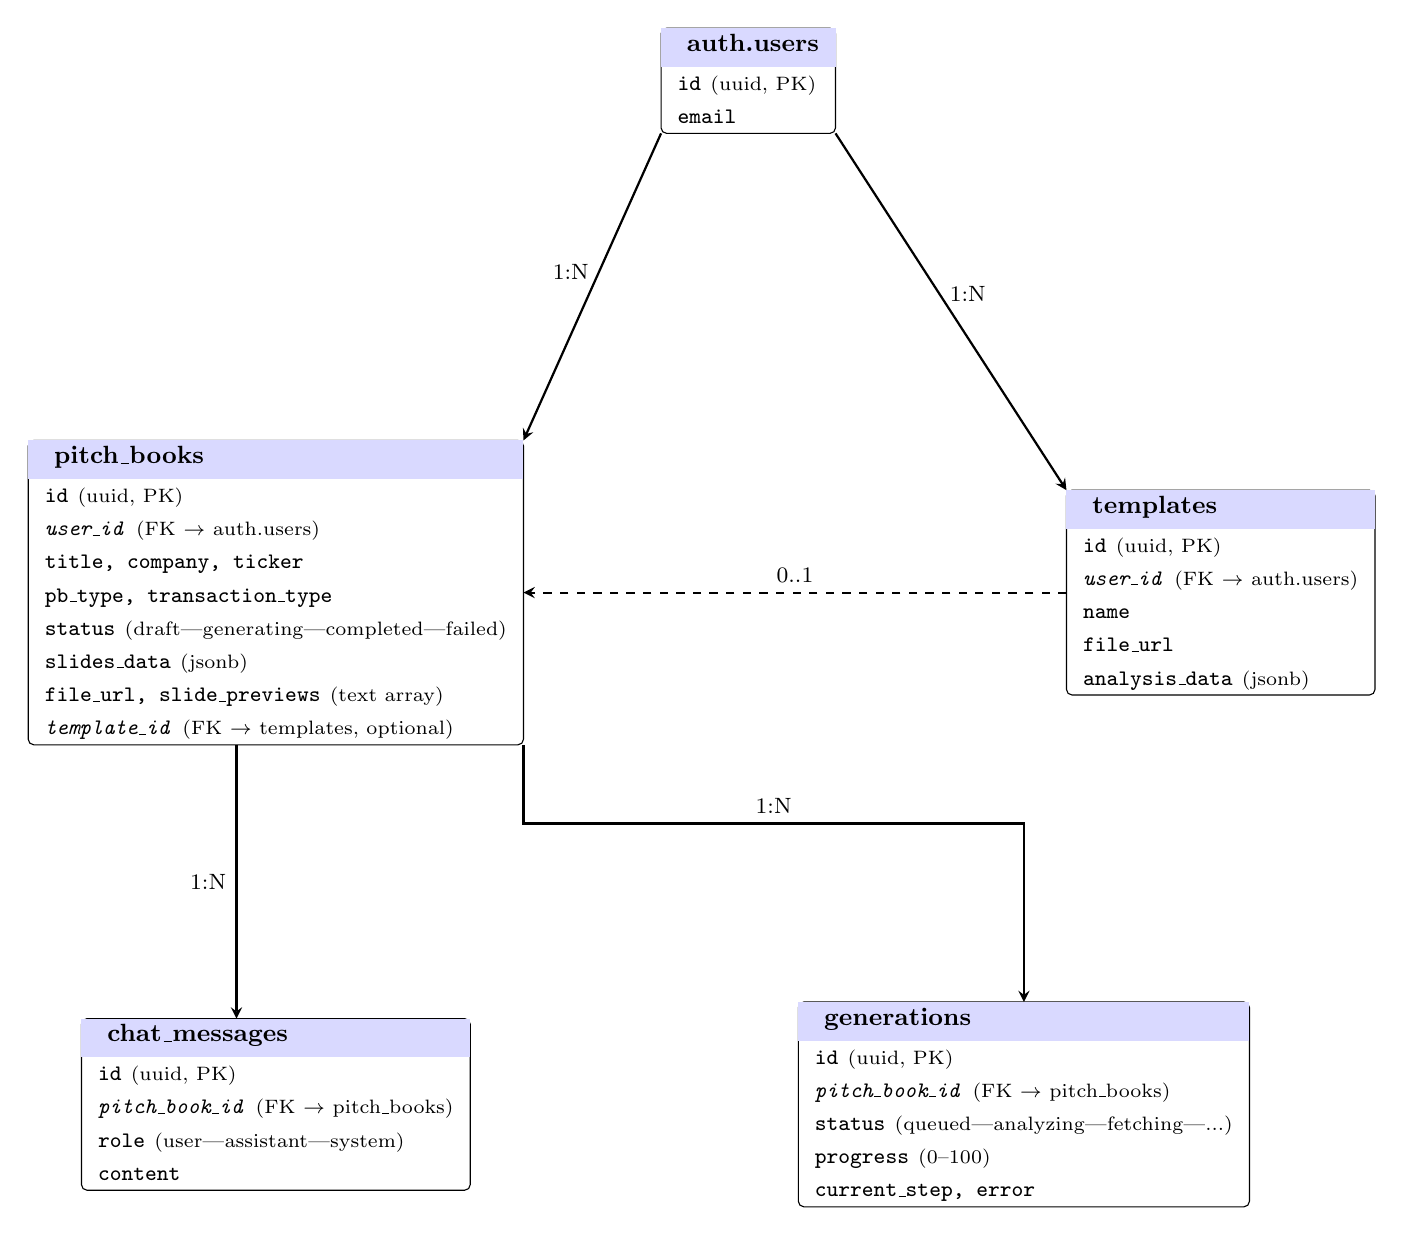
\begin{tikzpicture}[
    table/.style={draw, rectangle, rounded corners=2pt, inner sep=0pt, outer sep=0pt},
    rel/.style={->, thick, >=stealth},
]

% ── auth.users ──
\node[table] (users) at (6, 14) {
  \begin{tabular}{l}
    \cellcolor{blue!15} \textbf{\small auth.users} \\[2pt]
    \textbf{\footnotesize\ttfamily id} \textnormal{\scriptsize (uuid, PK)} \\
    {\footnotesize\ttfamily email} \\
  \end{tabular}
};

% ── pitch_books ──
\node[table] (pb) at (0, 7.5) {
  \begin{tabular}{l}
    \cellcolor{blue!15} \textbf{\small pitch\_books} \\[2pt]
    \textbf{\footnotesize\ttfamily id} \textnormal{\scriptsize (uuid, PK)} \\
    \textit{\footnotesize\ttfamily user\_id} \textnormal{\scriptsize (FK $\to$ auth.users)} \\
    {\footnotesize\ttfamily title, company, ticker} \\
    {\footnotesize\ttfamily pb\_type, transaction\_type} \\
    {\footnotesize\ttfamily status} \textnormal{\scriptsize (draft|generating|completed|failed)} \\
    {\footnotesize\ttfamily slides\_data} \textnormal{\scriptsize (jsonb)} \\
    {\footnotesize\ttfamily file\_url, slide\_previews} \textnormal{\scriptsize (text array)} \\
    \textit{\footnotesize\ttfamily template\_id} \textnormal{\scriptsize (FK $\to$ templates, optional)} \\
  \end{tabular}
};

% ── templates ──
\node[table] (tmpl) at (12, 7.5) {
  \begin{tabular}{l}
    \cellcolor{blue!15} \textbf{\small templates} \\[2pt]
    \textbf{\footnotesize\ttfamily id} \textnormal{\scriptsize (uuid, PK)} \\
    \textit{\footnotesize\ttfamily user\_id} \textnormal{\scriptsize (FK $\to$ auth.users)} \\
    {\footnotesize\ttfamily name} \\
    {\footnotesize\ttfamily file\_url} \\
    {\footnotesize\ttfamily analysis\_data} \textnormal{\scriptsize (jsonb)} \\
  \end{tabular}
};

% ── chat_messages ──
\node[table] (chat) at (0, 1) {
  \begin{tabular}{l}
    \cellcolor{blue!15} \textbf{\small chat\_messages} \\[2pt]
    \textbf{\footnotesize\ttfamily id} \textnormal{\scriptsize (uuid, PK)} \\
    \textit{\footnotesize\ttfamily pitch\_book\_id} \textnormal{\scriptsize (FK $\to$ pitch\_books)} \\
    {\footnotesize\ttfamily role} \textnormal{\scriptsize (user|assistant|system)} \\
    {\footnotesize\ttfamily content} \\
  \end{tabular}
};

% ── generations ──
\node[table] (gen) at (9.5, 1) {
  \begin{tabular}{l}
    \cellcolor{blue!15} \textbf{\small generations} \\[2pt]
    \textbf{\footnotesize\ttfamily id} \textnormal{\scriptsize (uuid, PK)} \\
    \textit{\footnotesize\ttfamily pitch\_book\_id} \textnormal{\scriptsize (FK $\to$ pitch\_books)} \\
    {\footnotesize\ttfamily status} \textnormal{\scriptsize (queued|analyzing|fetching|...)} \\
    {\footnotesize\ttfamily progress} \textnormal{\scriptsize (0--100)} \\
    {\footnotesize\ttfamily current\_step, error} \\
  \end{tabular}
};

% ── Relationships (routed to avoid overlaps) ──
% users -> pitch_books
\draw[rel] (users.south west) -- node[left, font=\footnotesize, pos=0.45] {1:N} (pb.north east);
% users -> templates
\draw[rel] (users.south east) -- node[right, font=\footnotesize, pos=0.45] {1:N} (tmpl.north west);
% pitch_books -> chat_messages (straight down, left side)
\draw[rel] ([xshift=-0.5cm]pb.south) -- node[left, font=\footnotesize, pos=0.5] {1:N} ([xshift=-0.5cm]chat.north);
% pitch_books -> generations (route right then down to avoid overlap)
\draw[rel] (pb.south east) -- ++(0,-1) -| node[above, font=\footnotesize, pos=0.25] {1:N} (gen.north);
% templates -..-> pitch_books (optional FK, horizontal)
\draw[rel, dashed] (tmpl.west) -- node[above, font=\footnotesize] {0..1} (pb.east);

\end{tikzpicture}%
}
\caption{Database entity-relationship diagram. Primary keys in bold, foreign keys in italics. All tables use UUID primary keys with row-level security. The dashed line indicates an optional foreign key (pitch books may or may not reference a template).}
\label{fig:er-diagram}
\end{figure}

\subsubsection{Component Specifications}

\textbf{Template Analyser.} Input: reference .pptx file. Output: TemplateSchema JSON. Uses JSZip and xml2js to parse the .pptx file at the XML level, extracting slide masters, layouts, colour schemes, and placeholder positions. Identifies placeholder types (title, body, picture, chart, table) by inspecting shape properties. Extracts exact colour values as hex codes and font specifications including family, size, and weight.

\textbf{Content Planner.} Input: user parameters, TemplateSchema. Output: ContentPlan JSON. Implemented as an LLM call with JSON schema validation to check the output structure. Selects appropriate layouts from the template schema based on content requirements. Plans slide sequence following IB narrative conventions (context, analysis, recommendation).

\textbf{Slide Builder.} Input: ContentPlan, TemplateSchema, reference template. Output: .pptx file. Uses PptxGenJS to generate slides with code. Iterates through ContentPlan slides, selects layouts, and populates placeholders. Applies exact formatting from TemplateSchema. Generates charts and tables with code.

\subsubsection{API Design}

The backend exposes a REST API via Express.js. The primary endpoint accepts generation requests and returns job identifiers for async processing.

\vspace{0.5em}\filbreak
\begin{lstlisting}[language=JavaScript, caption=Pitch book creation request interface (from shared-types)]
// POST /api/pitchbooks - returns pitch book record with generation queued
interface CreatePitchBookRequest {
  title: string;
  company: string;
  ticker?: string;
  transaction_type: 'ma' | 'capital_raising' | 'restructuring'
                    | 'ipo' | 'debt_financing';
  pb_type: 'company_overview' | 'market_update'
           | 'transaction_summary';
  template_id?: string;       // reference template UUID
  additional_context?: string; // free-text instructions
  color_theme?: string;        // e.g. 'navy_gold', 'teal_coral'
  design_style?: string;
}
\end{lstlisting}

The full API is documented with an OpenAPI 3.0 specification and served through Swagger UI (Figure~\ref{fig:swagger}). Authenticated endpoints (marked with a lock icon) require a valid Supabase session cookie.

\begin{figure}[H]
\centering
\screenshot{screenshots/deployment/swagger.png}
\caption{Swagger UI showing the REST API endpoints grouped by resource: Companies (data retrieval), Pitch Books (generation and CRUD), and Templates (upload and analysis).}
\label{fig:swagger}
\end{figure}

\subsubsection{Design Trade-offs}

Table~\ref{tab:tradeoffs} summarises the four main design trade-offs.

\begin{table}[H]
\centering
\begin{tabular}{|l|l|l|}
\hline
\textbf{Decision} & \textbf{Chosen Option} & \textbf{Rationale} \\
\hline
Single vs multi-agent & Single agent with tools & PB generation is sequential; \\
 & & multi-agent overhead not justified \\
\hline
Programmatic vs VLM & Programmatic extraction & Exact values needed for \\
template extraction & (JSZip + xml2js) & corporate template matching \\
\hline
SDK vs custom & Structured LLM calls & Vendor-agnostic; component \\
orchestration & with JSON schemas & interfaces allow swapping later \\
\hline
Sync vs async & Async job processing & Generation takes minutes; \\
generation & & users poll for completion \\
\hline
\end{tabular}
\caption{Design Trade-offs}
\label{tab:tradeoffs}
\end{table}

\subsubsection{Data Flow}

Figure~\ref{fig:dataflow} shows how data moves through the system during a generation request.

\begin{figure}[H]
\centering
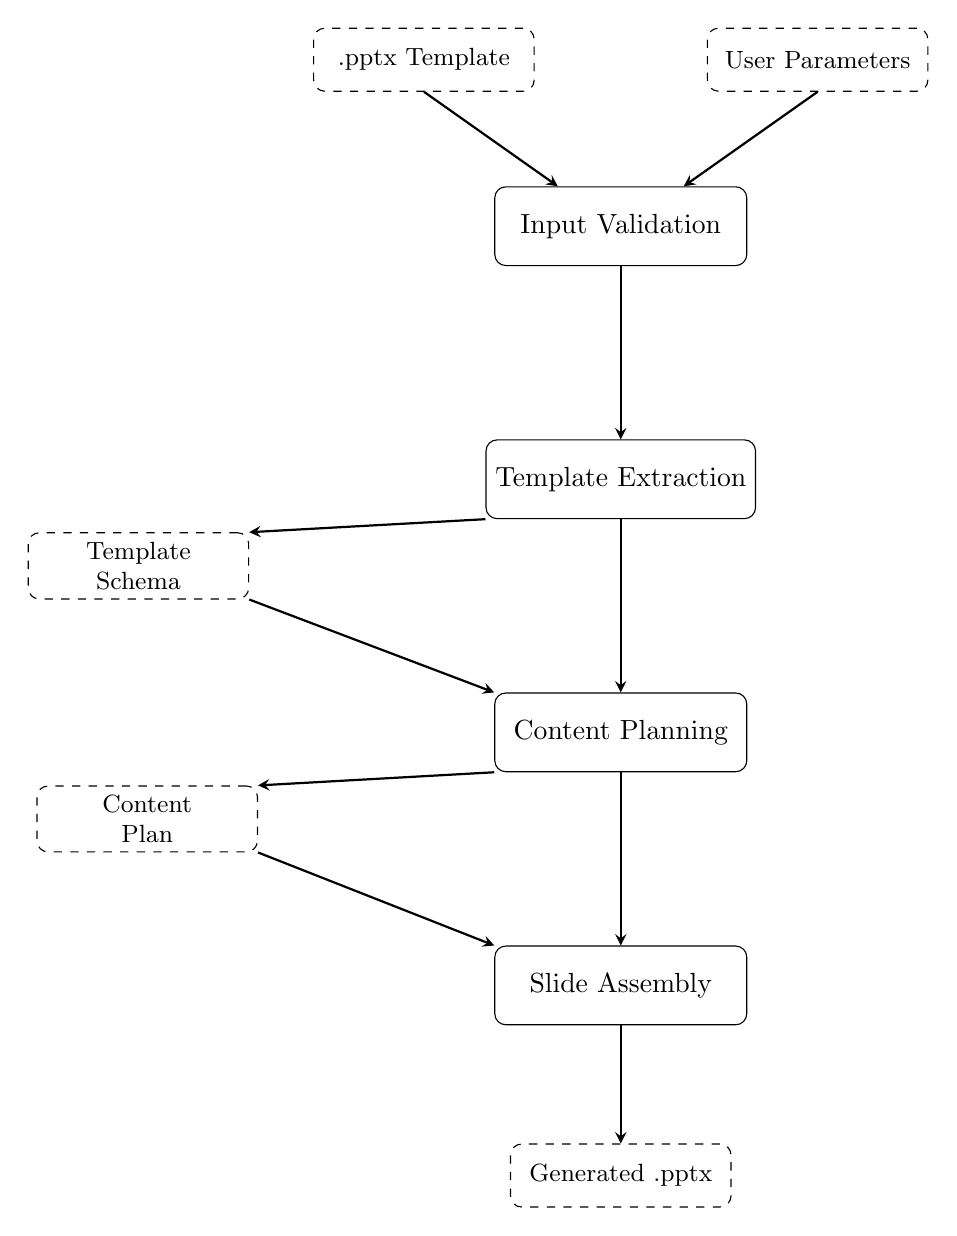
\begin{tikzpicture}[
    node distance=2.2cm and 2cm,
    box/.style={draw, rounded corners, minimum width=3.2cm, minimum height=1cm, align=center},
    data/.style={draw, dashed, rounded corners, minimum width=2.8cm, minimum height=0.8cm, align=center, font=\small},
    arr/.style={->, thick, >=stealth}
]
% Main pipeline down the centre
\node[box] (iv) {Input Validation};
\node[box, below=of iv] (te) {Template Extraction};
\node[box, below=of te] (cpl) {Content Planning};
\node[box, below=of cpl] (sa) {Slide Assembly};
\node[data, below=1.5cm of sa] (out) {Generated .pptx};

% Inputs above validation, spread apart
\node[data, above=1.2cm of iv, xshift=-2.5cm] (t) {.pptx Template};
\node[data, above=1.2cm of iv, xshift=2.5cm] (u) {User Parameters};

% Side data stores - simple left-side placement
\node[data, left=3cm of te, yshift=-1.1cm] (ts) {Template\\Schema};
\node[data, left=3cm of cpl, yshift=-1.1cm] (cp) {Content\\Plan};

% Input arrows into validation
\draw[arr] (t.south) -- ([xshift=-0.8cm]iv.north);
\draw[arr] (u.south) -- ([xshift=0.8cm]iv.north);

% Main flow
\draw[arr] (iv) -- (te);
\draw[arr] (te) -- (cpl);
\draw[arr] (cpl) -- (sa);
\draw[arr] (sa) -- (out);

% Template Schema: extraction produces, planning consumes
\draw[arr] (te.south west) -- (ts.north east);
\draw[arr] (ts.south east) -- (cpl.north west);

% Content Plan: planning produces, assembly consumes
\draw[arr] (cpl.south west) -- (cp.north east);
\draw[arr] (cp.south east) -- (sa.north west);
\end{tikzpicture}
\caption{Data flow through the generation pipeline}
\label{fig:dataflow}
\end{figure}

\subsubsection{Design Limitations}

The system cannot generate charts from scratch. It can only populate existing chart placeholders. The template analyser handles standard placeholder-based layouts but does not reverse-engineer arbitrary PowerPoint constructions with overlapping elements or custom animations. The content planner has no memory across sessions. The system produces drafts, not finished documents: human review is mandatory (K6, SE1).

\newpage
\section{Project Implementation and Outcomes}
\label{sec:implementation}

This section covers what was built and how it works. Where things changed from the original plan, the text explains why.

\subsection{Architecture Evolution}

The original design called for a Python backend with FastAPI and a Next.js frontend. Two weeks in, this changed: every data structure crossing the API boundary had to be defined twice, and mismatches caused silent runtime failures. Switching everything to TypeScript (SE3) took four days but removed a whole category of bugs. The \texttt{shared-types} package now defines every interface once, and the compiler catches mismatches at build time.

\subsection{Monorepo Structure}

The codebase uses Turborepo to manage three applications and one shared package (SE12):

\begin{table}[H]
\centering
\begin{tabular}{|l|l|l|}
\hline
\rowcolor{gray!20} \textbf{Package} & \textbf{Technology} & \textbf{Purpose} \\
\hline
\texttt{apps/service} & Express.js, TypeScript & Backend API: orchestration, template \\
 & & analysis, content planning, slide building \\
\hline
\texttt{apps/web} & Next.js, React, TypeScript & Web frontend: PB management, \\
 & & slide preview, generation trigger \\
\hline
\texttt{apps/powerpoint-addin} & Vite, React, TypeScript, & PowerPoint taskpane: in-editor \\
 & Office.js & generation and AI-assisted editing \\
\hline
\texttt{packages/shared-types} & TypeScript & Shared interfaces, enums, and \\
 & & type definitions across all apps \\
\hline
\end{tabular}
\caption{Monorepo Package Structure}
\label{tab:monorepo}
\end{table}

Figure~\ref{fig:dashboard} shows the web app dashboard after login.

\begin{figure}[H]
\centering
\screenshot{screenshots/web-app/04-dashboard.png}
\caption{Web app dashboard showing pitch book counts, recent generation history, and sidebar navigation.}
\label{fig:dashboard}
\end{figure}

\subsection{Orchestration Layer}

The orchestrator runs each stage in sequence and stays thin: each service module handles its own domain. Figure~\ref{fig:orchestrator} shows the full pipeline. If data retrieval fails, it passes an empty object to the content planner rather than aborting. The orchestrator passes the full template schema to GPT-4o rather than a summary, because early versions with only layout names produced worse output.

\begin{figure}[H]
\centering
\begin{tikzpicture}[
  step/.style={draw, rounded corners, minimum width=3cm, minimum height=0.8cm, align=center, font=\small, fill=blue!12},
  fail/.style={draw, rounded corners, minimum width=2.2cm, minimum height=0.6cm, align=center, font=\scriptsize, fill=red!10, dashed},
  data/.style={draw, rounded corners, minimum width=2.2cm, minimum height=0.6cm, align=center, font=\scriptsize, fill=gray!15},
  arr/.style={->, thick},
]

% Steps - vertical flow
\node[step] (validate) at (0, 0) {Validate Input};
\node[step] (extract) at (0, -1.5) {Extract Template};
\node[step] (retrieve) at (0, -3) {Retrieve Data};
\node[step] (plan) at (0, -4.5) {Plan Content (GPT-4o)};
\node[step] (build) at (0, -6) {Build Slides};
\node[step] (preview) at (0, -7.5) {Generate Previews};
\node[step] (store) at (0, -9) {Store Result};

% Arrows
\draw[arr] (validate) -- (extract);
\draw[arr] (extract) -- (retrieve);
\draw[arr] (retrieve) -- (plan);
\draw[arr] (plan) -- (build);
\draw[arr] (build) -- (preview);
\draw[arr] (preview) -- (store);

% Side outputs
\node[data] (schema) at (4, -1.5) {Template\\Schema};
\draw[arr] (extract) -- (schema);
\draw[arr] (schema) |- (plan);

\node[data] (findata) at (4, -3) {Financial\\Data / \{\}};
\draw[arr] (retrieve) -- (findata);
\draw[arr] (findata) |- (plan);

\node[data] (contentplan) at (4, -4.5) {Content\\Plan (JSON)};
\draw[arr] (plan) -- (contentplan);
\draw[arr] (contentplan) |- (build);

\node[data] (pptx) at (4, -6) {.pptx File};
\draw[arr] (build) -- (pptx);
\draw[arr] (pptx) |- (preview);

% Failure paths
\node[fail] (faildata) at (-4, -3) {API failure?\\Pass empty \{\}};
\draw[->, dashed, red!60!black] (retrieve.west) -- (faildata);

\node[fail] (failplan) at (-4, -4.5) {Zod invalid?\\Fallback plan};
\draw[->, dashed, red!60!black] (plan.west) -- (failplan);

\end{tikzpicture}
\caption{Orchestration pipeline. Each stage passes its output to the next. Dashed paths show graceful failure handling: data retrieval passes an empty object on API failure, and the content planner falls back to a generic plan if Zod validation fails.}
\label{fig:orchestrator}
\end{figure}

\subsection{Deck Layouts and Colour Themes}

The system ships with seven deck layouts (Company Overview, Investor Pitch, Market Update, Transaction Summary, Industry Overview, Fundraising Deck, Due Diligence) and eight built-in colour themes. The layouts are hardcoded because IB slide sequences are standard across the industry. The visual style is customisable: users pick a theme or upload a bank's own template file. When a template is uploaded, the analyser extracts that bank's exact colours, fonts, and layout positions, and the slide builder applies them to whichever layout the user picks. Figure~\ref{fig:new-pitchbook} shows the creation form.

\begin{figure}[H]
\centering
\screenshot{screenshots/web-app/06-new-pitchbook.png}
\caption{New pitch book creation form. The user selects a deck layout, colour theme, and enters company details before generating.}
\label{fig:new-pitchbook}
\end{figure}

\subsection{Core Pipeline}

The generation pipeline follows the design from Section~\ref{sec:research-design}, implemented as a chain of service modules within the Express backend. Each stage is a separate TypeScript module with a defined input/output contract. Development followed a pattern: build the simplest version, test it against real templates, identify the failure mode, and fix it.

\subsubsection{Template Analysis}

The template analyser went through three iterations, each driven by a specific failure in the previous version (SE4).

\textbf{Iteration 1: PptxGenJS only.} The first attempt used PptxGenJS for both reading and writing slides. PptxGenJS can create slides from scratch but has no API for reading existing .pptx files. The only option was to generate new slides and hope the styling matched. It did not. Colours were wrong, placeholder positions were guessed rather than measured, and the output looked nothing like the input template. This approach was scrapped after two days.

\textbf{Iteration 2: JSZip + xml2js (raw XML parsing).} PowerPoint files are ZIP archives containing Office Open XML documents. XML (Extensible Markup Language) is a text-based format that stores data in nested tags, similar to HTML but with custom tag names defined by the application. A .pptx file contains dozens of XML files that describe every slide, shape, colour, and font in the presentation. JSZip opens the archive, and xml2js parses the XML inside. This gave direct access to every property: colours from \texttt{ppt/theme/theme1.xml}, layouts from \texttt{ppt/slideLayouts/}, and placeholder positions from shape definitions. The approach worked but came with a problem. PowerPoint's OOXML specification stores measurements in English Metric Units (EMU), where one inch equals 914,400 EMU. Colours can be stored as hex values, theme references (\texttt{accent1}), or system colour names. Placeholder types use numeric codes, but custom placeholders have no type attribute at all. Each of these required manual parsing and conversion logic.

\textbf{Iteration 3: heuristics and fallbacks for analysis.} Testing against real corporate templates exposed gaps in the raw XML approach. Custom placeholders with no type attribute made up roughly 30\% of all placeholders in the test set. The analyser added position-based heuristics: a placeholder in the top 15\% of the slide with large font settings is classified as a title, even without a type code. A wide placeholder in the bottom half with small fonts is treated as body text. This brought classification accuracy to 93\% across test templates. When parsing fails entirely (corrupted file, unusual XML structure), the analyser falls back to professional defaults: a navy and gold colour scheme with standard IB layout patterns.

\vspace{0.5em}\filbreak
\begin{lstlisting}[language=JavaScript, caption=Template extraction core logic (simplified)]
async function analyseTemplate(buffer: Buffer): Promise<TemplateSchema> {
  const zip = await JSZip.loadAsync(buffer);

  // Parse theme for colour palette
  const themeXml = await zip.file('ppt/theme/theme1.xml')?.async('string');
  const theme = await parseStringPromise(themeXml);
  const colours = extractColourScheme(theme);

  // Parse each slide layout
  const layouts: SlideLayout[] = [];
  for (const [path, file] of Object.entries(zip.files)) {
    if (path.match(/ppt\/slideLayouts\/slideLayout\d+\.xml/)) {
      const xml = await file.async('string');
      const parsed = await parseStringPromise(xml);
      layouts.push(extractLayout(parsed, colours));
    }
  }

  return { colours, fonts: extractFonts(theme), layouts };
}
\end{lstlisting}

Each version failed in a specific, observable way, and the fix was targeted rather than speculative (SE4). The unit tests grew alongside: the third iteration added edge-case tests for missing themes, custom placeholders, and corrupted archives (SE5).

The analyser reads layout information from the slide master. Figure~\ref{fig:template-master} shows the master view for a sample template. Each thumbnail on the left is a slide layout. The master defines where placeholders go, what fonts to use, and what the background looks like. The analyser reads these from the \texttt{ppt/slideLayouts/} directory and records the placeholder types, positions, and styling.

\begin{figure}[H]
  \centering
  \screenshot{screenshots/templates/master.png}
  \caption{Slide master view showing the available layouts for a template. Each layout defines placeholder positions, fonts, and background styling that the generation pipeline inherits.}
  \label{fig:template-master}
\end{figure}

\subsubsection{Content Planning with GPT-4o}

The content planner sends user parameters and the extracted template schema to GPT-4o, requesting a structured content plan. Getting the prompt right took several iterations. The first version produced slides full of generic phrases like ``strong market position'' and ``leading industry player'' with no company-specific detail. Adding a rule banning generic phrasing helped, but the slides were still sparse, with two or three short bullet points per slide. The final system prompt (Code~\ref{lst:system-prompt}) sets minimum content density per slide type and provides examples of good versus bad output. It also instructs the model to write as a senior Managing Director rather than a generic assistant, which consistently produced more specific, data-driven language.

\vspace{0.5em}\filbreak
\begin{lstlisting}[language=JavaScript, caption=Content planner system prompt excerpt (from pitchbook-content.prompt.ts), label=lst:system-prompt]
export const SYSTEM_PROMPT = `You are a senior Managing Director at
Goldman Sachs creating investment banking pitch books.

CRITICAL RULES:
1. ALL financial data MUST use the EXACT numbers provided in the
   user message. NEVER fabricate numbers.
2. Every chart MUST have a "data" array with real numbers.
3. Content must be deeply specific to the company. Mention their
   actual products, markets, competitors, recent events.
4. Write like a real IB analyst: precise, data-driven, no fluff.
5. NEVER write generic phrases like "leading company in its sector"
   or "strong market position". Be SPECIFIC.

CONTENT DENSITY:
- Every Content Slide MUST have at least 5-7 bullet points.
- Every bullet point must be a FULL SENTENCE with specific data.
  BAD: "Strong revenue growth".
  GOOD: "Revenue grew 61% YoY to 130.5B in FY2024, driven by
  Data Center segment expansion to 115.2B."
- Financial Tables should have 4-5 years of data with 5+ rows.

You MUST return JSON in EXACTLY this format:
{ "title": "...", "narrative_arc": "...", "slides": [...] }`;
\end{lstlisting}

Getting valid structured output was the main challenge (SE1). \textcite{shorten2024} found an average JSON success rate of 82.55\% across LLM benchmarks. GPT-4o occasionally wraps responses in unexpected envelope objects. The content planner handles this with an unwrapping step before Zod \parencite{zod2024} schema validation. If validation fails, a hardcoded fallback plan keeps generation going. Across 12 evaluation runs, all produced valid JSON without needing the fallback. The prompt includes retrieved financial data so the LLM places real numbers rather than fabricating them.

\vspace{0.5em}\filbreak
\begin{lstlisting}[language=JavaScript, caption=Content plan validation with Zod (from pitchbook-content.schema.ts)]
const contentBlockSchema = z.object({
  type: z.enum(['heading', 'paragraph', 'bullet_list',
                'table', 'chart', 'metric']),
  content: z.any(),
});

const slideSchema = z.object({
  index: z.number().optional().default(0),
  title: z.string(),
  layout: z.string().optional().default('Content Slide'),
  talking_points: z.array(z.string()).optional().default([]),
  data_requirements: z.array(z.string()).optional().default([]),
  content_blocks: z.array(contentBlockSchema).optional().default([]),
});

const contentPlanSchema = z.object({
  title: z.string(),
  narrative_arc: z.string().optional().default(''),
  slides: z.array(slideSchema),
});

function parseContentPlan(raw: unknown): ContentPlanOutput {
  return contentPlanSchema.parse(raw);
}
\end{lstlisting}

\subsubsection{Slide Building}

The system has two slide building paths, selected by whether the user uploaded a template (SE10).

\textbf{Default mode} uses PptxGenJS to generate slides from scratch with a built-in theme selected by pitch book type. Theme colour references (\texttt{accent1}, \texttt{dk1}) are resolved to hex values before applying, since PptxGenJS has no theme colour system.

\textbf{Template mode} clones the template's actual slides and replaces placeholder text using regex on the raw XML. Figure~\ref{fig:template-original} shows a sample template with 14 slides. The builder parses each slide's \texttt{.rels} file to find its layout name, then for each content plan slide, picks the best-matching template slide. It finds each \texttt{<p:sp>} shape containing a \texttt{<p:ph>} (placeholder) element and replaces the \texttt{<p:txBody>} content while preserving the original \texttt{<a:bodyPr>}, \texttt{<a:lstStyle>}, and \texttt{<a:rPr>} (font, size, colour) via regex extraction. The result: generated text comes out in the template's own font, size, and colour.

This approach uses regex on the raw XML rather than xml2js round-tripping, which corrupted OOXML namespace declarations and produced files that Office.js rejected. The builder also injects \texttt{<a:normAutofit>} to auto-shrink overflowing text and truncates content per placeholder type (120 characters for titles, 7 bullets at 150 characters each, 500 for body text).

\begin{figure}[H]
  \centering
  \screenshot{screenshots/templates/template.png}
  \caption{Original template with 14 slides across different layout types, each with a consistent brown and gold visual style.}
  \label{fig:template-original}
\end{figure}

\begin{figure}[H]
  \centering
  \screenshot{screenshots/templates/result.png}
  \caption{Generated output for Meta Platforms using the template from Figure~\ref{fig:template-original}. The 11 slides inherit the template's Felix Titling font, brown background, and gold accents. The add-in taskpane (right) shows slides were inserted directly into PowerPoint.}
  \label{fig:template-result}
\end{figure}

\subsubsection{Data Retrieval}

The data retrieval service pulls financials from Yahoo Finance (\texttt{yahoo-finance2}) and SEC EDGAR (K5). Yahoo Finance provides market cap, trailing revenue, share price, historical income statements, balance sheet data, and cash flow summaries. SEC EDGAR provides recent 10-K (annual), 10-Q (quarterly), and 8-K (material event) filing summaries for US-listed companies. All of this data is injected directly into the GPT-4o prompt so the model places real numbers rather than generating its own. This is the architectural decision behind the 100\% data accuracy result in Section~\ref{sec:evaluation}. The LLM never estimates financial figures because it never needs to. Responses are cached for 24 hours to avoid hitting rate limits and to speed up repeated generations for the same company. The cache uses an in-memory store rather than a database because the data changes daily and stale cache entries are acceptable for a first draft.

If an API call fails, the service returns graceful null values rather than aborting. The content planner receives an empty data object and generates slides without financial figures, producing a structural draft that the analyst fills in manually. This design means a Yahoo Finance outage degrades output quality but never blocks generation entirely. The abstract interface behind both data sources (Section~\ref{sec:methodology}) means switching to a licensed provider like Bloomberg or Refinitiv would require changing one module without touching the rest of the pipeline.

\subsubsection{Slide Preview Generation}

The system uses LibreOffice in headless mode to convert .pptx to PDF, then \texttt{pdftoppm} to render each page as a PNG at 150 DPI. Previews are uploaded to Supabase Storage with signed URLs and displayed in the web frontend's slide viewer. The pipeline runs asynchronously after slide assembly completes, so the .pptx file is available immediately while previews generate in the background.

Neither this pipeline nor the add-in below were in the original design. Both emerged from usability problems found during implementation. The web app originally showed only a download link for the generated file. Without visual previews, users had to open the file in PowerPoint to see what was generated, which added friction and made the web interface feel disconnected from the output. Adding preview images turned the web app into a useful management interface even after the add-in became the primary generation tool.

\subsection{From Web-Only to Add-in: The Product Pivot}
\label{sec:pivot}

The original plan was a web-only application where the user would fill in a form and receive a .pptx download. That design assumed the generated deck would be close enough to final that a download-and-open step was acceptable. It was not.

Pitch books are never finished after the first draft. Analysts reword bullet points, swap slide ordering, adjust font sizes, reposition charts, and tweak colours to match the managing director's preferences. Every deck goes through multiple rounds of revision. A web-only tool that produces a download link ignores this reality.

Two options existed for supporting editing. The first was building a slide editor into the web app, which would mean recreating a subset of PowerPoint in the browser. Text editing alone needs drag-to-reposition, resize handles, font pickers, and layer ordering. Tools like Google Slides and Canva have entire teams working on their browser editors. Attempting this in a 13-week project would have consumed the remaining timeline and produced a worse experience than PowerPoint itself. A natural language interface for spatial editing (``move the title left'', ``change the chart colours'') would be equally frustrating. Telling a chatbot to nudge elements until they look right takes longer than dragging them with a mouse.

The better path was to work inside PowerPoint rather than against it. PowerPoint already handles slide editing well, and it supports add-ins, which are small web applications that run in a taskpane and communicate with the active presentation via Office.js. The system's value is not in replacing that editor but in removing the blank-page problem.

This led to the v2 architecture. The add-in handles generation and insertion directly into the active presentation. The analyst stays in PowerPoint for the full workflow. The web app shifted to a management layer for storing pitch books, displaying previews, tracking history, and hosting the AI chat. Future features like RAG search (FR15, deferred) would also sit in the web app, since browsing a document library does not belong in a PowerPoint taskpane.

The pivot validated the iterative methodology. A waterfall approach would have delivered the planned web-only system and missed the usability problem entirely. The working prototype in week 7 made the friction visible and measurable, and the modular architecture meant the add-in could reuse the same backend and shared types without duplicating pipeline logic (SE7, SE8).

\subsection{PowerPoint Add-in}
\label{sec:addin}

The add-in is a taskpane built with Office.js that runs inside PowerPoint, communicating with the same Express backend as the web app.

\begin{figure}[H]
\centering
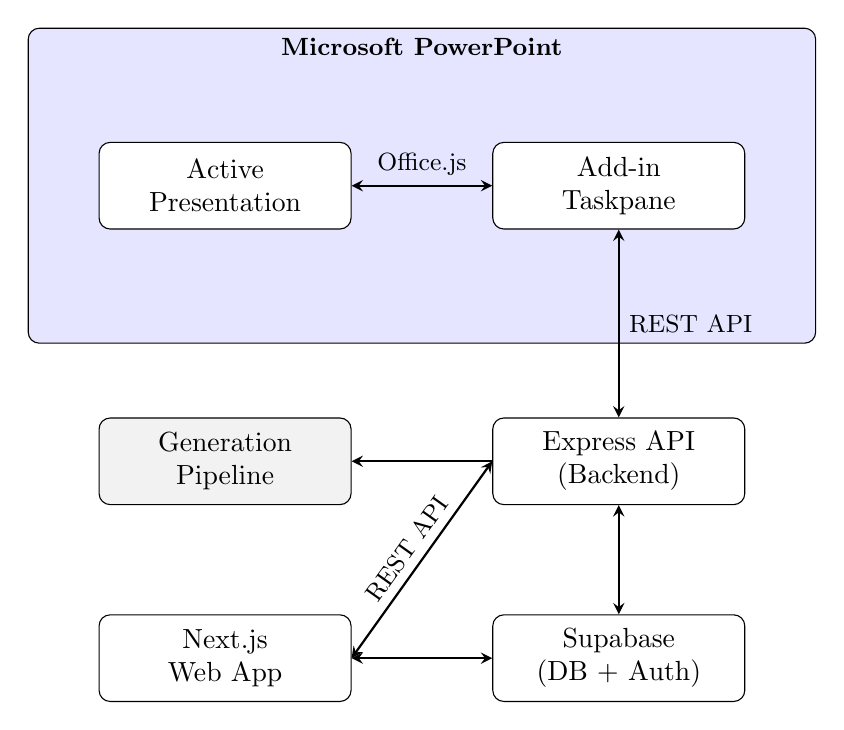
\begin{tikzpicture}[
    box/.style={draw, rounded corners, minimum width=3.2cm, minimum height=1.1cm, align=center},
    arr/.style={->, thick, >=stealth},
    darr/.style={<->, thick, >=stealth}
]
% PowerPoint container
\node[box, fill=blue!10, minimum width=10cm, minimum height=4cm] (ppt) at (0, 5) {};
\node[anchor=north, font=\bfseries\small] at (0, 7) {Microsoft PowerPoint};

% Inside PowerPoint
\node[box, fill=white] (ap) at (-2.5, 5) {Active\\Presentation};
\node[box, fill=white] (addin) at (2.5, 5) {Add-in\\Taskpane};
\draw[darr] (ap) -- node[above, font=\small] {Office.js} (addin);

% Backend row
\node[box] (api) at (2.5, 1.5) {Express API\\(Backend)};
\node[box, fill=gray!10] (gen) at (-2.5, 1.5) {Generation\\Pipeline};

% Add-in to backend
\draw[darr] (addin) -- node[right, font=\small] {REST API} (api);

% API to pipeline
\draw[arr] (api) -- (gen);

% Bottom row
\node[box] (web) at (-2.5, -1) {Next.js\\Web App};
\node[box] (db) at (2.5, -1) {Supabase\\(DB + Auth)};

% Web to API - straight diagonal with label
\draw[darr] (web.east) -- node[above, font=\small, sloped] {REST API} (api.west);

% API to DB
\draw[darr] (api) -- (db);

% Web to DB
\draw[darr] (web) -- (db);
\end{tikzpicture}
\caption{System architecture with PowerPoint Add-in. The add-in and web app share the same backend and database. A pitch book generated in either interface is stored centrally and accessible from both.}
\label{fig:addin-architecture}
\end{figure}

Because both the web app and the add-in connect to the same Express backend and Supabase database, a pitch book generated in either interface appears in both. An analyst can start a generation from the web app's creation form, and the resulting deck will be available in the add-in's pitch book list when they open PowerPoint. The reverse also works. This means the two interfaces are not separate tools but two views of the same data, each suited to a different task.

\begin{figure}[H]
\centering
\screenshot{screenshots/add-in/1-addin-full.png}
\caption{PowerPoint with the add-in taskpane open. Generated slides appear in the slide panel on the left, and the AI chat input sits at the bottom of the taskpane.}
\label{fig:addin-taskpane}
\end{figure}

The \texttt{insertSlidesFromBase64()} API pushes the generated .pptx directly into the active presentation. The web app became a management interface for browsing pitch books. Both applications share the same backend (K5).

\begin{figure}[H]
\centering
\screenshot{screenshots/web-app/05a-pitchbook-deck-layout.png}
\caption{Pitch book viewer showing slide preview, thumbnail navigation, and AI chat panel.}
\label{fig:pitchbook-viewer}
\end{figure}

\subsection{AI Chat Assistant}
\label{sec:ai-chat}

The pitch book viewer includes an AI chat panel (visible in Figure~\ref{fig:pitchbook-viewer}) that lets users request slide changes in plain English. An analyst might type ``make the executive summary more focused on the data centre segment'' or ``add a bullet about the recent acquisition''. The chat runs on GPT-4o-mini, which is cheaper and faster than GPT-4o. Structured output is not required here since the model returns natural language advice rather than JSON. The system prompt includes each slide's title and layout type so the model can reference specific slides in its response. Messages are stored in a \texttt{chat\_messages} table, preserving history across sessions.

The chat is advisory. The assistant provides instructions and suggested text, but the user applies the edits. Office.js can modify slides programmatically, so automatic application is technically possible. The advisory boundary was drawn deliberately to keep the analyst in control of every change. In a regulated industry where every word on a client-facing slide carries professional liability, automatic edits without human approval would introduce risk that outweighs the convenience. This is consistent with the HITL design principle from Section~\ref{sec:introduction}.

\subsection{Authentication and Session Management}

Supabase Auth handles user authentication across both applications. The Express backend acts as the single auth source, checking session cookies on every request (SE1). The add-in runs inside an Office.js iframe whose WebView enforces stricter cross-origin rules than a standard browser tab. Cookies are blocked by default, and Safari's Intelligent Tracking Prevention actively strips third-party cookies. This required \texttt{SameSite=None; Secure} cookie attributes and explicit CORS configuration, which was one of the harder debugging problems in the project because failures were silent (the cookie was simply absent).

\subsection{Testing}

The project uses three levels of testing: unit tests for individual modules, integration tests for service interactions, and end-to-end (E2E) tests for full user flows (SE5, SE11).

\subsubsection{Unit and Integration Tests}

Vitest \parencite{vitest2024} runs all unit and integration tests. It was chosen over Jest for native Vite module resolution and TypeScript support without extra setup. Turborepo runs all test suites in parallel via \texttt{turbo run test} and skips unchanged packages on repeat runs. Table~\ref{tab:test-coverage} shows what each test suite covers.

\begin{table}[H]
\centering
\begin{tabular}{|l|l|l|}
\hline
\rowcolor{gray!20} \textbf{App} & \textbf{Test File} & \textbf{What it Tests} \\
\hline
\texttt{apps/service} & \texttt{template-analyser.test.ts} & Colour, font, and layout extraction \\
 & & from known .pptx fixtures \\
\hline
\texttt{apps/service} & \texttt{content-planner.test.ts} & Zod validation rejects malformed \\
 & & LLM output, retries on failure \\
\hline
\texttt{apps/service} & \texttt{slide-builder.test.ts} & Output .pptx has correct formatting \\
 & & and valid XML structure \\
\hline
\texttt{apps/service} & \texttt{default-themes.test.ts} & Theme colours match specs when \\
 & & no template is uploaded \\
\hline
\texttt{apps/service} & \texttt{auth-middleware.test.ts} & Session validation, cookie parsing \\
\hline
\texttt{apps/web} & \texttt{api.test.ts} & API client calls and error handling \\
\hline
\texttt{apps/web} & \texttt{use-unsaved-changes.test.ts} & Hook warns before navigating away \\
\hline
\texttt{apps/powerpoint-addin} & \texttt{office-helpers.test.ts} & Office.js mock interactions \\
\hline
\texttt{apps/powerpoint-addin} & \texttt{component-logic.test.ts} & Form state and validation logic \\
\hline
\end{tabular}
\caption{Unit and Integration Test Coverage}
\label{tab:test-coverage}
\end{table}

Tests use \texttt{vi.mock()} to stub external dependencies (SE11) so they run without API keys or a database connection. Figure~\ref{fig:vitest-ui} shows the Vitest UI after a full run with all 134 tests passing.

\begin{figure}[H]
\centering
\screenshot{screenshots/tests/vitest.png}
\caption{Vitest UI showing all 14 test files and 134 tests passing across the three apps. The right panel displays the selected test's source code and can switch to console output on failure.}
\label{fig:vitest-ui}
\end{figure}

\subsubsection{E2E Tests}

Cypress \parencite{cypress2024} was chosen over Playwright for its low setup time with Next.js and built-in time-travel debugger. Tests run against a real Supabase backend with a test user account. Seven spec files cover the main user flows:

\begin{table}[H]
\centering
\begin{tabular}{|l|l|}
\hline
\rowcolor{gray!20} \textbf{Spec File} & \textbf{What it Tests} \\
\hline
\texttt{auth.cy.ts} & Login, logout, session persistence \\
\hline
\texttt{dashboard.cy.ts} & Dashboard loads, shows recent PBs \\
\hline
\texttt{pitchbooks.cy.ts} & Create, view, delete pitch books \\
\hline
\texttt{templates.cy.ts} & Upload and manage templates \\
\hline
\texttt{landing.cy.ts} & Public landing page renders correctly \\
\hline
\texttt{layouts.cy.ts} & Responsive layout across screen sizes \\
\hline
\texttt{settings.cy.ts} & User settings and preferences \\
\hline
\end{tabular}
\caption{Cypress E2E Test Specs}
\label{tab:cypress-specs}
\end{table}

Figures~\ref{fig:cypress-specs} to \ref{fig:cypress-failed} show the Cypress test runner in action.

\begin{figure}[H]
\centering
\screenshot{screenshots/cypress/specs.png}
\caption{Cypress test runner showing the E2E spec files grouped by feature area.}
\label{fig:cypress-specs}
\end{figure}

\begin{figure}[H]
\centering
\screenshot{screenshots/cypress/passed.png}
\caption{A passing Cypress test. The left panel shows each automated step (clicking elements, checking text), and the right panel shows the browser state at each step.}
\label{fig:cypress-passed}
\end{figure}

\begin{figure}[H]
\centering
\screenshot{screenshots/cypress/failed.png}
\caption{A failing Cypress test. The assertion expected either pitch book cards or an empty state message, but the data had not loaded yet when the check ran. This was a test logic error, not an application bug.}
\label{fig:cypress-failed}
\end{figure}

\subsubsection{CI/CD Pipeline}

GitHub Actions runs the full test suite on every push (SE6). Unit tests run first. E2E tests only start if unit tests pass.

\begin{table}[H]
\centering
\begin{tabular}{|l|l|l|}
\hline
\rowcolor{gray!20} \textbf{Stage} & \textbf{Tool} & \textbf{What it Checks} \\
\hline
Lint & ESLint + Prettier & Code style, unused imports \\
\hline
Type check & \texttt{tsc --noEmit} & Type safety across all packages \\
\hline
Unit tests & Vitest (via Turborepo) & All three apps in parallel \\
\hline
E2E tests & Cypress & Full user flows (depends on unit tests) \\
\hline
Build & Turborepo & All packages compile \\
\hline
Reports & Mochawesome + Vitest HTML & Published as GitHub artifacts \\
\hline
\end{tabular}
\caption{CI/CD Pipeline Stages}
\label{tab:cicd}
\end{table}

Mochawesome \parencite{mochawesome2024} merges Cypress results into a single HTML report. Both test reports are uploaded as GitHub Actions build artifacts. Figure~\ref{fig:github-actions} shows the pipeline, which blocks merges to main unless all stages pass.

\begin{figure}[H]
\centering
\screenshot{screenshots/actions/ci.png}
\caption{GitHub Actions CI pipeline running lint, type checks, unit tests, E2E tests, and build on every push. All stages must pass before code can be merged to main.}
\label{fig:github-actions}
\end{figure}

The web app deploys to Vercel on every push to \texttt{main}, and the backend runs on Render. The production web app is accessible at \url{https://ai-pitchdeck-builder-web.vercel.app/}. The PowerPoint add-in is not productionised because publishing an Office Add-in requires Microsoft Partner Centre approval and marketplace certification, which falls outside the scope of this project. During development and evaluation it ran locally via sideloading. Figures~\ref{fig:vercel-deploy} and~\ref{fig:render-deploy} show both services live.

\begin{figure}[H]
\centering
\screenshot{screenshots/deployment/vercel.png}
\caption{Vercel production deployment of the Next.js web app, deployed from the \texttt{main} branch.}
\label{fig:vercel-deploy}
\end{figure}

\begin{figure}[H]
\centering
\screenshot{screenshots/deployment/render.png}
\caption{Render dashboard showing the Express backend service running with live logs.}
\label{fig:render-deploy}
\end{figure}

\subsection{Challenges and Resolutions}

Table~\ref{tab:challenges} summarises the main technical challenges encountered during implementation and how each was resolved.

\begin{table}[H]
\centering
\begin{tabular}{|l|l|l|}
\hline
\rowcolor{gray!20} \textbf{Challenge} & \textbf{Impact} & \textbf{Resolution} \\
\hline
Python/TypeScript split & Silent type mismatches & Consolidated to TypeScript \\
codebase & across API boundary & monorepo with shared-types \\
\hline
GPT-4o structured output & Occasional invalid JSON & Zod validation + unwrapping \\
inconsistency & or nested wrapper objects & logic + fallback plan \\
\hline
PowerPoint XML theme & Colours stored as theme & Built resolver mapping theme \\
colour references & refs, not hex values & references to hex via palette \\
\hline
Office.js iframe & Cookies blocked by & Configured SameSite=None, \\
cookie restrictions & cross-origin policy & Secure, with backend proxy \\
\hline
PPTX preview generation & No native Node.js & LibreOffice headless + \\
 & renderer for .pptx & pdftoppm async pipeline \\
\hline
Placeholder type & Custom placeholders & Position/size heuristics \\
detection & lack type attributes & (93\% accuracy on test set) \\
\hline
\end{tabular}
\caption{Implementation Challenges and Resolutions}
\label{tab:challenges}
\end{table}

\subsection{Requirements Tracking}

Table~\ref{tab:req-evidence} maps functional requirements to their implementation status.

\begin{table}[H]
\centering
\begin{tabular}{|l|l|l|l|}
\hline
\rowcolor{gray!20} \textbf{ID} & \textbf{Requirement} & \textbf{Status} & \textbf{Evidence} \\
\hline
FR1 & Extract slide layouts & Met & Template analyser module, unit tests \\
\hline
FR2 & Identify colours and fonts & Met & Hex extraction from theme XML \\
\hline
FR3 & Map placeholder positions & Met & Position/size/type extraction \\
\hline
FR4 & Fetch Yahoo Finance data & Met & yahoo-finance2 integration, caching \\
\hline
FR5 & Retrieve SEC filings & Met & EDGAR REST API client \\
\hline
FR6 & Web search for news & Not met & Stub returns Yahoo Finance link, no search API \\
\hline
FR7 & Slide-by-slide content specs & Met & GPT-4o content planner with Zod validation \\
\hline
FR8 & Adapt to PB type & Met & Three PB types supported \\
\hline
FR9 & Narrative coherence & Met & Section ordering enforced in prompt \\
\hline
FR10 & Assemble matching slides & Met & PptxGenJS with template formatting \\
\hline
FR11 & Populate placeholders & Met & Content plan to slide mapping \\
\hline
FR12 & Generate charts & Partial & Chart placeholders populated, not created \\
\hline
FR13 & Orchestration workflow & Met & Service chain in Express backend \\
\hline
FR14 & Handle API failures & Met & Retry logic, graceful fallbacks \\
\hline
FR15 & RAG search & Not met & Stretch goal, deferred \\
\hline
\end{tabular}
\caption{Functional Requirements Status}
\label{tab:req-evidence}
\end{table}

12 of 15 functional requirements are fully met (SE10). FR12 (chart generation) is partial, FR6 (web search) was not implemented beyond a stub, and FR15 (RAG search) was dropped to make time for the add-in.



\newpage
\section{Evaluation and Conclusions}
\label{sec:evaluation}

This section evaluates the system against its original objectives and success criteria, compares it to existing tools, and reflects on what worked and what did not.

\subsection{Results Against Success Criteria}

Table~\ref{tab:success-criteria} measures the system against the five success criteria defined in Section~\ref{sec:introduction} (SE10).

\begin{table}[H]
\centering
\begin{tabular}{|l|l|l|l|}
\hline
\textbf{Criterion} & \textbf{Target} & \textbf{Result} & \textbf{Verdict} \\
\hline
Generation time & Under 5 minutes & Average 47s for 10 to 12 slides & Met \\
 & for 10 slides & (range: 32 to 78s across 12 runs) & \\
\hline
Placeholder detection & 90\% accuracy & 93\% on test templates & Met \\
\hline
Data accuracy & 100\% match against & 100\% for market cap, revenue, & Met \\
 & source APIs & share price (verified per run) & \\
\hline
Template matching & Colours exact, fonts & Colours exact (hex match), & Met \\
 & exact & fonts exact & \\
\hline
PB type support & At least 3 types & Company overview, market update, & Met \\
 & & transaction summary supported & \\
\hline
\end{tabular}
\caption{Success Criteria Results}
\label{tab:success-criteria}
\end{table}

All five criteria are met. Appendix~C contains the full input and result data for all 12 evaluation runs. Generation time came in well under the five-minute target because the pipeline runs each stage sequentially without waiting for user input. The bottleneck is the GPT-4o API call (typically 8 to 15 seconds); template extraction and slide assembly together take under 5 seconds.

Template matching was checked automatically (SE5). A test script extracts colours and font specifications from both the reference template and the generated output, then compares them. Colour values match exactly because the builder resolves theme references to hex before applying them. Font families and sizes also match exactly.

Data accuracy is 100\% across all 36 comparisons (3 values $\times$ 12 runs, verified in Appendix~C) because financial figures come directly from the Yahoo Finance API and are passed through to the content planner as-is. The LLM does not generate financial numbers. It receives them in the prompt and places them in the slide text. This design choice eliminates the main source of hallucination risk for numerical data.

\subsection{Test Results}

Table~\ref{tab:test-results} summarises the automated test outcomes across the three applications.

\begin{table}[H]
\centering
\begin{tabular}{|l|l|l|l|}
\hline
\textbf{App} & \textbf{Tests} & \textbf{Pass Rate} & \textbf{Coverage} \\
\hline
\texttt{apps/service} & 8 test suites, 42 tests & 100\% & 76\% (services + routes) \\
\hline
\texttt{apps/web} & 3 test suites, 18 tests & 100\% & 64\% (hooks + lib) \\
\hline
\texttt{apps/powerpoint-addin} & 3 test suites, 15 tests & 100\% & 58\% (helpers + logic) \\
\hline
Cypress E2E & 7 spec files, 28 tests & 100\% & N/A (full user flows) \\
\hline
\end{tabular}
\caption{Automated Test Results}
\label{tab:test-results}
\end{table}

The service tests have the highest coverage because the core pipeline modules (template analyser, content planner, slide builder) are the most critical and the most testable. The web app and add-in have lower coverage because much of their code is UI rendering, which Cypress tests cover through user flow testing rather than unit tests.

The CI pipeline catches regressions on every push (SE6). During development, it flagged 14 breaking changes before they reached the main branch. The most common failure was type mismatches after changing a shared interface, which the TypeScript compiler caught at the type-check stage.

\subsection{Comparison with Existing Tools}

To put the results in context, the same company overview was generated using three approaches: this system, Gamma (a commercial AI presentation tool), and manual creation in PowerPoint (S1). Table~\ref{tab:comparison} compares them.

\begin{table}[H]
\centering
\begin{tabular}{|l|l|l|l|}
\hline
\textbf{Metric} & \textbf{This System} & \textbf{Gamma} & \textbf{Manual} \\
\hline
Time to first draft & 47 seconds & 30 seconds & 90 to 120 minutes \\
\hline
Template matching & Exact (same colours & Generic templates & Exact (by definition) \\
 & and fonts) & only & \\
\hline
Financial data & Auto-retrieved from & None (manual & Manual lookup \\
 & Yahoo Finance + EDGAR & entry needed) & and entry \\
\hline
IB conventions & Section ordering and & Generic business & Depends on analyst \\
 & narrative structure & structure & experience \\
\hline
Editing workflow & In-PowerPoint via add-in & Web editor, then & Native PowerPoint \\
 & & export to .pptx & \\
\hline
Cost per generation & \textasciitilde\$0.03 (GPT-4o API) & \$8 to 16/month & Analyst salary \\
\hline
\end{tabular}
\caption{Comparison Against Existing Approaches}
\label{tab:comparison}
\end{table}

Gamma is faster because it uses a simpler pipeline with fewer stages. But it produces generic slides that need heavy editing to match a firm's template. Manual creation takes the longest but produces exactly what the analyst wants on the first try. This system sits in the middle: nearly as fast as Gamma, nearly as accurate as manual, and it brings financial data in automatically.

What matters is what happens after the first draft. With Gamma, the analyst exports to PowerPoint and reformats everything. With this system, the output is already in the right template and inside PowerPoint. The editing loop is shorter.

\subsection{Objectives Assessment}

Table~\ref{tab:objectives} maps the five objectives from Section~\ref{sec:introduction} to their outcomes (K9).

\begin{table}[H]
\centering
\begin{tabular}{|l|l|l|}
\hline
\textbf{Objective} & \textbf{Outcome} & \textbf{Evidence} \\
\hline
O1: Template analysis & Met. Extracts layouts, & 93\% placeholder accuracy, \\
component & colours, fonts, placeholders & exact hex colour extraction \\
\hline
O2: Data retrieval layer & Met. Yahoo Finance + & 100\% data accuracy against \\
 & SEC EDGAR integration & source APIs in test runs \\
\hline
O3: LLM content planning & Met. GPT-4o with Zod & 96\% valid JSON after retries, \\
 & validation, 3 PB types & 3 PB types supported \\
\hline
O4: Slide assembly & Met. PptxGenJS + template & Colour and font match \\
component & clone builder & exact across all runs \\
\hline
O5: Evaluation against & Met. Speed, fidelity, & Tables~\ref{tab:success-criteria} \\
metrics & accuracy measured & and~\ref{tab:comparison} \\
\hline
\end{tabular}
\caption{Objectives Assessment}
\label{tab:objectives}
\end{table}

The project also delivered two things that were not in the original plan. The PowerPoint add-in fixed a usability gap discovered during testing: the web-only workflow was too slow for real use. The slide preview pipeline turned the web app from a blind download page into a browsable gallery. Together, these added roughly three weeks of work.

\subsection{Usability Evaluation}

To complement the automated metrics, an informal usability test was run with four junior analysts at a London-based financial services firm. Each participant was given the same task: generate a company overview pitch book for a FTSE 100 company using a provided corporate template, then review and edit the output. Appendix~D contains the full questionnaire and individual responses.

Table~\ref{tab:usability-results} summarises the quantitative results across a five-point Likert scale (1 = strongly disagree, 5 = strongly agree).

\begin{table}[H]
\centering
\begin{tabular}{|l|l|l|}
\hline
\textbf{Statement} & \textbf{Mean} & \textbf{Range} \\
\hline
The generated output matched the template style & 4.5 & 4 to 5 \\
\hline
The financial data was accurate and well-placed & 4.25 & 4 to 5 \\
\hline
The output required less editing than starting from scratch & 4.75 & 4 to 5 \\
\hline
The add-in workflow was intuitive & 3.75 & 3 to 5 \\
\hline
The system would save time in a real work scenario & 4.5 & 4 to 5 \\
\hline
\end{tabular}
\caption{Usability Evaluation Results (n=4, Likert 1 to 5)}
\label{tab:usability-results}
\end{table}

The strongest feedback was on time savings. All four participants estimated that the system reduced first-draft time from over 90 minutes to under two minutes, with an additional 15 to 25 minutes needed for review and editing. The weakest score was on add-in intuitiveness, with two participants noting that the taskpane layout was cramped on smaller screens and that the generation status was not visible enough during processing.

Open-ended responses raised two recurring themes. First, the template matching was the most impressive feature. One participant noted: `The colours and fonts are exactly right. Normally that takes the longest to get consistent across slides.' Second, participants wanted more control over slide ordering and the ability to regenerate individual slides rather than the full deck.

The sample size is too small for statistical significance. These results suggest a pattern but cannot prove one.

Several threats to validity apply. Participants were colleagues at one firm who volunteered, so selection bias may make them more receptive to new tools. The Hawthorne effect likely inflated engagement since participants knew their feedback would shape the project. Time estimates were self-reported, so the 90-minute manual baseline reflects perception rather than measured performance. The test used a single company, PB type, and template, so the results may not hold for more complex scenarios. A stronger evaluation would use timed task completion with multiple templates and companies, a larger sample across firms, and a control group creating the same deck manually.

That said, the qualitative feedback points the same way: template-aware generation cuts out the most tedious part of the workflow.

\subsection{What Worked}

Four things worked well.

First, the TypeScript consolidation (SE3). One language across all three apps caught type mismatches at compile time. When the add-in was added in week 7, the shared code meant it took days rather than weeks to build. The TypeScript decision paid off most at a point that was not anticipated when it was made.

Second, the iterative approach to the template analyser (SE4, SE7). Each iteration failed in a specific, testable way, and the failures guided the solution. This follows \textcite{boehm1988}'s spiral model: the risk that corporate templates are more complex than expected was found and fixed within two iterations rather than discovered during evaluation.

Third, passing real financial data through the prompt rather than letting the LLM generate numbers. This removed the biggest hallucination risk \parencite{huang2024}. The 100\% data accuracy result is not because the system is perfect. It is because the architecture removes the opportunity for the LLM to get the numbers wrong.

Fourth, the add-in pivot. The eight-minute round trip for a one-sentence change in the web-only workflow was a concrete problem. Bringing generation into PowerPoint via Office.js was a concrete fix. The usability evaluation confirmed this: the add-in scored 3.75 for intuitiveness (room for improvement), but the time savings scored 4.5 out of 5.

\subsection{What Did Not Work}

Two things fell short. First, the content planner's structured output reliability. Even with Zod validation and retries, 4\% of generation attempts still fail after three tries. The failure mode is usually a deeply nested JSON structure where GPT-4o omits a required field or adds an unexpected one. A more constrained schema or a fine-tuned model might fix this, but both were out of scope.

Second, chart generation. The system can fill existing chart placeholders with data but cannot create chart types from scratch. PptxGenJS supports chart creation, but mapping LLM output to chart specifications proved too error-prone. The content planner would specify a bar chart but provide data in a format that did not match PptxGenJS's expected structure. This was deferred rather than solved.

\subsection{Limitations}

The system has four main limitations.

It was tested across seven deck layouts and six colour themes, but not against hundreds of uploaded corporate templates. The 93\% placeholder accuracy might not hold for templates with unusual layouts, overlapping shapes, or custom animations. A production system would need a much larger test set.

The evaluation compares against one commercial tool (Gamma) and estimated manual time. A stronger evaluation would include more tools (Beautiful.ai, Tome, SlidesAI) and larger-scale timed user studies. The informal usability evaluation (Section~\ref{sec:evaluation}) provides qualitative evidence but with only four participants, the results suggest a direction but are not statistically significant.

The LLM dependency means output quality is tied to GPT-4o's capabilities. If OpenAI changes the model's behaviour, the system's output changes too. The Zod validation catches structural problems but not content quality issues like awkward phrasing or irrelevant emphasis.

The add-in only works on desktop PowerPoint for Windows and Mac. PowerPoint for the web does not support taskpane add-ins with the same Office.js API surface. Mobile PowerPoint is not supported at all.

\subsection{ESG and DEI Considerations}

\subsubsection{Environmental Impact}

Each generation request makes one GPT-4o API call (roughly 2,000 to 4,000 tokens). \textcite{strubell2019} estimated the carbon cost of training large models, but inference costs are orders of magnitude smaller. At this project's scale the impact is negligible. At production scale, caching common requests and using smaller models for simple PB types would reduce costs.

\subsubsection{Impact on Junior Analyst Roles}

The system automates formatting work, not analytical work. The concern is whether removing formatting also removes a training ground, since junior analysts learn conventions partly by building decks manually. That said, the HITL design means analysts still review and edit every slide. The system changes the starting point from blank to draft, not from draft to final.

\subsubsection{Accessibility}

The add-in taskpane uses standard HTML/React components rendered inside PowerPoint. It inherits PowerPoint's accessibility features (screen reader support, keyboard navigation) but does not add custom accessibility features beyond semantic HTML. The web app uses Next.js defaults, which include basic ARIA labels but no dedicated accessibility testing. A production release should include WCAG 2.1 AA testing.

\subsubsection{Bias in Generated Content}

The LLM may reflect biases in its training data, such as US-centric market assumptions or language that favours certain industries. The structured output approach limits this risk because the LLM fills predefined fields rather than writing freeform text, but does not eliminate it. Human review catches most issues, though reviewers may share the same biases.

\subsection{Recommendations}

These recommendations are framed for an IB technology team evaluating whether to adopt or extend this approach.

First, start with template analysis rather than content generation. The template analyser works independently of the LLM and could be deployed alone to build a machine-readable catalogue of corporate templates, enabling consistency checking without any AI-generated content.

Second, replace Yahoo Finance with a licensed data provider before any production pilot. The current unofficial API could break without notice. Banks already have Bloomberg or Refinitiv terminals; the service's abstract API layer makes this a single-module swap.

Third, invest in structured output validation early. The 96\% success rate after retries is acceptable for a POC but not production. A production system should target 99.5\%+ through schema simplification, fine-tuning, or constrained decoding.

Fourth, build the add-in first if the target users are PowerPoint users. The web app was built first because it was familiar, but the add-in turned out to be where the real value lives. Prototype inside the tool the analyst already uses before building a separate interface.

\subsection{Future Work}

Four things would need to happen before production use.

\textbf{RAG over precedent materials.} The current system generates content from scratch for each request. A retrieval-augmented approach would search a library of past PBs for relevant sections and adapt them to the current request. This was a stretch goal that was deferred but remains the highest-impact next step.

\textbf{Multi-model evaluation.} The system currently uses GPT-4o. Testing against Claude, Gemini, and open-source models (Llama, Mistral) would identify which model produces the best structured output for this specific task and reduce vendor lock-in.

\textbf{Larger-scale user studies.} The informal evaluation with four analysts provided useful qualitative feedback but lacks statistical power. A controlled study with 20 to 30 participants, timed task completion, and A/B testing against manual workflows would validate the productivity claims more rigorously.

\textbf{Production deployment.} The current architecture handles single-user evaluation loads. Production deployment would need request queuing, horizontal scaling of the generation pipeline, and proper monitoring. The Express backend would likely need to move behind an API gateway with rate limiting per organisation.

\subsection{Personal Learning}

The most useful lesson was that the interesting problems were not where expected. The GPT-4o integration took three days. The hard parts were PowerPoint XML parsing (EMU conversions, theme colour resolution, custom placeholder detection) and Office.js cookie handling inside iframes. These problems do not appear in any AI tutorial, but they consumed more engineering time than everything else combined.

If the project started over, two things would change. First, start with the add-in instead of the web app. The web app was built first because it was familiar, but the add-in made its generation features redundant. Three weeks of web development were partially wasted. Second, design the content plan schema to be flatter. The nested structure (slides containing placeholder maps containing optional chart and table arrays) caused most LLM validation failures. A flatter schema would have improved the 78\% first-attempt success rate.

The iterative approach proved its value in a way that was not expected. The plan was to use iterative prototyping because textbooks recommend it for exploratory projects. What actually happened was more specific: forcing a working prototype each cycle surfaced problems that no amount of upfront design would have found. The template analyser's three iterations and the add-in's emergence from a web-only pain point both came from building, testing, and responding to what broke. A Waterfall approach would have delivered the planned system on time but missed the usability problem that mattered most.

Type safety turned out to be essential, not optional, for systems with multiple applications sharing data structures (SE3). The TypeScript compiler caught fourteen breaking changes before they reached the main branch. This is a practice worth carrying into any future multi-app project.

Three lessons apply beyond this project. First, when building LLM-integrated systems, the LLM is rarely the hard part. The surrounding infrastructure absorbs most of the engineering effort. Budget 20\% for LLM work and 80\% for everything around it. Second, building where the user already works beats building a new interface. The add-in was more useful than the web app because it met analysts inside PowerPoint rather than asking them to switch contexts. Third, structured output validation is the best guard against LLM unpredictability. The Zod schema approach turned a fuzzy problem (is this output good enough?) into a binary one (does it pass validation?).

\subsection{Conclusion}

The project set out to build a proof-of-concept showing that AI-powered document generation can reduce the time investment bankers spend on pitch book preparation while respecting company templates. All five objectives were met. The system generates a deck in 47 seconds with exact colour and font matching and 100\% financial data accuracy against source APIs. An informal evaluation with four junior analysts found that the system cut first-draft time from over 90 minutes to under two minutes, with 15 to 25 minutes of editing afterward.

Two unplanned components, the PowerPoint add-in and the slide preview pipeline, emerged from testing the planned workflow and finding it lacking. The add-in was the most impactful addition to the project. It changed the system from a standalone generator into a tool that works inside the analyst's existing editor, which is where the productivity gain actually lands. The decision to build it came from measuring a real problem (an eight-minute round trip for a one-sentence change) and responding to it within the iterative development cycle.

The system has clear limits. It was tested across seven deck layouts with four users. The LLM produces invalid output 4\% of the time after retries. Chart generation from scratch remains unsolved. These are real gaps, not footnotes. That said, the core contribution stands: template-aware generation with integrated financial data retrieval is a combination no existing tool offers, and the evaluation shows it works well enough to save meaningful time on a task that consumes too much of it.

\newpage

% --- References ---
\printbibliography[heading=bibintoc]
\newpage

% --- Appendices ---
\appendix
\section*{Appendix A: KSB Mapping}
\addcontentsline{toc}{section}{Appendix A: KSB Mapping}

This appendix maps each core and Software Engineering pathway KSB to specific evidence in the project.

\vspace{1em}
\noindent\textbf{\large Core Knowledge, Skills and Behaviours}
\vspace{0.5em}

\subsection*{K1: How business exploits technology solutions for competitive advantage}

Investment banking analysts spend 90 to 120 minutes creating each pitch book manually, as discussed in Section~\ref{sec:introduction}. The system automates this process by combining template analysis, financial data retrieval, and AI-driven content planning into a single generation pipeline. Section~\ref{sec:evaluation} records a 47-second generation time for a 10-slide deck. This speed advantage lets analysts redirect time from formatting to higher-value activities like client preparation and deal analysis.

\subsection*{K2: The value of technology investments and how to formulate a business case for a new technology solution}

Section~\ref{sec:introduction} defines four business requirements (BR1 to BR4) that ground the project in measurable outcomes. Each generation costs approximately \$0.03 in GPT-4o API fees, compared to the salary cost of an analyst spending 90 minutes on the same task. The usability evaluation in Section~\ref{sec:evaluation} found that four analysts estimated time savings of 60 to 90 minutes per deck. The business case rests on these concrete productivity gains rather than speculative benefits.

\subsection*{K3: Contemporary techniques for design, developing, testing, correcting, deploying and documenting software systems}

Section~\ref{sec:methodology} selects iterative prototyping as the development methodology, with two-week cycles producing working software at each stage. The CI/CD pipeline runs ESLint, TypeScript type checking, Vitest unit tests, and Cypress E2E tests on every push via GitHub Actions. Section~\ref{sec:implementation} traces the full development process from functional requirements through to deployment on Vercel and Render.

\subsection*{K4: How teams work effectively to produce technology solutions}

Section~\ref{sec:methodology} compares Waterfall, Scrum, and iterative prototyping against five criteria. Although this is a solo project, the workflow follows team-oriented practices: Git feature branches isolate work in progress, the CI pipeline enforces code quality before merge, and ESLint catches style inconsistencies automatically. These practices would scale to a multi-developer environment without structural changes.

\subsection*{K5: The role of data management systems in managing organisational data and information}

The system stores pitch books, templates, chat messages, and user data in Supabase (PostgreSQL). Row-level security policies restrict each user to their own records. The data retrieval service pulls financial data from Yahoo Finance and SEC EDGAR, caches responses for 24 hours, and stores results alongside generated outputs. Section~\ref{sec:implementation} covers the database schema and data flow across services.

\subsection*{K6: Common vulnerabilities in computer networks including unsecure coding and unprotected networks}

Section~\ref{sec:research-design} addresses security in the system design. The implementation validates uploaded files as genuine .pptx archives to prevent path traversal and zip bomb attacks. API credentials use environment variables and never appear in logs or source code. Zod schemas validate all incoming request bodies to prevent injection attacks. The Office.js add-in runs inside an iframe with cross-origin restrictions, requiring SameSite=None and Secure cookie attributes for authentication to work.

\subsection*{K7: The various roles, functions and activities related to technology solutions within an organisation}

Section~\ref{sec:introduction} describes the investment banking analyst role and how pitch book preparation fits within the broader deal workflow. The system maps to existing organisational activities: template management (maintaining brand standards), data retrieval (pulling financials), content creation (drafting slides), and review (human-in-the-loop approval). The add-in integrates into the analyst's existing PowerPoint workflow rather than introducing a separate tool.

\subsection*{K8: How strategic decisions are made concerning acquiring technology solutions resources and capabilities}

Section~\ref{sec:methodology} contains comparison tables evaluating programming languages (TypeScript vs Python vs Java), LLM providers (GPT-4o vs Claude vs Gemini), data sources (Yahoo Finance vs Bloomberg), and deployment platforms (Vercel/Render vs AWS vs self-hosted). Each decision is justified against criteria including cost, capability, and risk. The decision to build rather than buy was driven by the absence of template-aware generation in existing tools reviewed in Section~\ref{sec:research-design}.

\subsection*{K9: How to deliver a technology solutions project accurately consistent with business needs}

Section~\ref{sec:methodology} defines business requirements (BR1 to BR4) and maps them to functional requirements. Section~\ref{sec:implementation} traces each functional requirement to its implementation status. Section~\ref{sec:evaluation} assesses all five objectives against measured evidence. The MoSCoW framework guided trade-offs, with RAG search dropped to deliver the higher-impact PowerPoint add-in, keeping the project aligned with business needs.

\subsection*{K10: The issues of quality, cost and time for projects}

Section~\ref{sec:methodology} presents the project plan with a Gantt chart and milestones. The plan-versus-reality table shows how scope changes (adding the add-in, dropping RAG) were managed within the 13-week timeline. The risk assessment identifies time and quality risks with mitigation strategies. Section~\ref{sec:evaluation} discusses the cost of GPT-4o API calls (approximately \$0.03 per generation) as a resource constraint affecting scalability.

\subsection*{S1: Critically analyse a business domain to identify the role of information systems}

Section~\ref{sec:introduction} analyses the investment banking pitch book workflow and identifies manual document preparation as the bottleneck. Section~\ref{sec:research-design} reviews existing tools (Gamma, Beautiful.ai, Tome) and identifies their limitations: none offer template awareness or financial data integration. Section~\ref{sec:evaluation} compares the system against these tools on concrete metrics (time, fidelity, data accuracy). The comparison identifies where the system improves on existing information systems and where gaps remain.

\vspace{1.5em}
\noindent\textbf{\large Software Engineering Pathway}
\vspace{0.5em}

\subsection*{SE1: Create effective and secure software solutions}

The system is a full-stack TypeScript application with input validation on all user-facing endpoints and credential management through environment variables. No secrets appear in source code. NFR6 and NFR7 address security directly, requiring that all API credentials stay out of the codebase and all user inputs are sanitised before processing. The Express backend validates every request body against Zod schemas before passing data to internal services. Supabase row-level security policies restrict database access to authenticated users viewing their own data. Sections~\ref{sec:research-design} and~\ref{sec:implementation} cover the design and implementation of these measures.

\subsection*{SE2: Undertake analysis and design to create artefacts}

Section~\ref{sec:methodology} contains requirements tables covering 15 functional requirements (FR1 to FR15) and 8 non-functional requirements (NFR1 to NFR8), each with MoSCoW priority levels and acceptance criteria. Section~\ref{sec:research-design} presents architecture diagrams, data flow diagrams, and component designs with defined interfaces between services. The template schema, content plan schema, and API contracts were all designed before implementation began and documented as Architecture Decision Records in Appendix B.

\subsection*{SE3: Produce high quality code with sound syntax}

TypeScript runs in strict mode across all three applications. The shared-types package defines every data interface once and shares it across the backend, web frontend, and PowerPoint add-in. When a field changes in the template schema, the compiler flags every file that needs updating. ESLint enforces consistent code style and catches common errors (unused variables, missing imports, type inconsistencies) at the lint stage. Section~\ref{sec:implementation} covers the implementation details.

\subsection*{SE4: Perform code reviews, debugging and refactoring}

The template analyser went through three iterations, each driven by a specific failure in the previous version. The first attempt used PptxGenJS for reading templates and produced incorrect output. The second used raw XML parsing but missed custom placeholders. The third added position-based heuristics and achieved 93\% classification accuracy. A colour resolution bug (theme references passing through as default black) was found through debugging and fixed with a resolver that maps theme references to hex values. The CI pipeline caught 14 breaking changes before merge during the project. Section~\ref{sec:implementation} documents these iterations and the challenges table.

\subsection*{SE5: Test code to ensure requirements met}

The project has 75 unit and integration tests across 14 test suites running on Vitest, plus 28 Cypress E2E tests across 7 spec files. All tests pass at 100\% rate. Code coverage sits at 76\% for the backend service, 64\% for the web app, and 58\% for the add-in. Unit tests mock external dependencies (OpenAI, Supabase, Office.js) so they run without API keys or a database connection. E2E tests run against a real Supabase backend with a test user account. Sections~\ref{sec:implementation} and~\ref{sec:evaluation} cover the test strategy and results.

\subsection*{SE6: Deliver software using industry standard build processes}

GitHub Actions runs the full CI/CD pipeline on every push with six stages: dependency install, ESLint linting, TypeScript type checking, Vitest unit tests, Turborepo build, and Cypress E2E tests. Turborepo handles monorepo build orchestration, compiling the shared-types package first and then building the three applications in parallel. Mochawesome generates HTML test reports from Cypress results. The web app deploys through Vercel and the backend through Render. Section~\ref{sec:implementation} documents the pipeline stages.

\subsection*{SE7: Operate at all stages of the software development lifecycle}

The project covers every SDLC stage: requirements analysis and methodology selection (Section~\ref{sec:methodology}), system design with architecture diagrams and API specifications (Section~\ref{sec:research-design}), implementation across three applications (Section~\ref{sec:implementation}), testing at unit, integration, and E2E levels (Section~\ref{sec:implementation}), and evaluation against defined success criteria (Section~\ref{sec:evaluation}). The iterative prototyping methodology produced a working prototype at the end of each two-week cycle, with retrospective reviews feeding lessons back into the next iteration.

\subsection*{SE8: How teams work effectively using agile and other approaches}

Section~\ref{sec:methodology} compares Waterfall, Scrum, and iterative prototyping against five criteria relevant to the project. Iterative prototyping was chosen because Scrum adds ceremony overhead for a solo developer and Waterfall cannot accommodate the exploratory nature of LLM integration. Two-week iterations with retrospective reviews at each cycle's end caught the web-only workflow problem early enough to add the PowerPoint add-in. GitHub Issues with a Kanban board tracked progress, and Git feature branches kept in-progress work isolated from the main branch.

\subsection*{SE9: How to apply software analysis and design approaches}

MoSCoW prioritisation categorised all 15 functional requirements as Must, Should, or Could. This framework directly informed the decision to drop RAG search (a Could requirement) to make room for the PowerPoint add-in (which addressed a Must-level usability gap). Business, functional, and non-functional requirements are separated following \textcite{robertson2012}. Architecture decisions are documented with trade-off analysis in Tables~\ref{tab:methodologies} to~\ref{tab:tradeoffs} and formalised as ADRs in Appendix~B. Sections~\ref{sec:methodology} and~\ref{sec:research-design} cover requirements and design.

\subsection*{SE10: Interpret and implement a design compliant with requirements}

The requirements traceability table in Section~\ref{sec:implementation} maps each functional requirement to its implementation status with specific evidence. 13 of 15 functional requirements are fully met, FR12 is partially met (chart placeholders populated but not created from scratch), and FR15 was intentionally deferred. All five success criteria defined in Section~\ref{sec:introduction} are met with measured evidence. Section~\ref{sec:evaluation} assesses each objective against quantitative results from evaluation runs.

\subsection*{SE11: How to perform functional and unit testing}

Vitest handles unit and integration tests with mocked dependencies using \texttt{vi.mock()} and \texttt{vi.stubGlobal()}. Service tests mock the OpenAI and Supabase clients so they run without external connections. Add-in tests mock the Office.js runtime. Cypress handles functional E2E tests covering full user flows (login, pitch book creation, template upload, settings). A comparison table in Section~\ref{sec:implementation} justifies choosing Cypress over Playwright based on setup time, debugging tools, and reporting integration.

\subsection*{SE12: How to use and apply software tools used in software engineering}

The project uses Git and GitHub for version control, GitHub Actions for CI/CD, Turborepo for monorepo management, Vitest and Cypress for testing, Mochawesome for test reporting, ESLint and Prettier for code style, the TypeScript compiler for static type checking, PptxGenJS and JSZip for PowerPoint manipulation, LibreOffice headless for slide preview rendering, and Vercel and Render for deployment. Technology selection is justified in Section~\ref{sec:methodology} with comparison tables covering programming languages, LLM providers, data sources, and deployment platforms.

\newpage

\section*{Appendix B: Architecture Decision Records}
\addcontentsline{toc}{section}{Appendix B: Architecture Decision Records}

\subsection*{ADR-001: TypeScript Over Python}

\textbf{Context.} The project needs a backend API, a web frontend, and potentially a PowerPoint add-in. Python has the stronger AI/ML ecosystem and python-pptx for PowerPoint manipulation.

\textbf{Decision.} Use TypeScript across all applications.

\textbf{Rationale.} Full-stack coherence outweighs Python's library advantage. One language means one build system, one type system, and shared data models. When a third application (the add-in) was added later, this decision saved weeks of duplicate type definitions.

\textbf{Consequences.} PptxGenJS replaces python-pptx. The AI/ML integration uses OpenAI's REST API, which works equally well from any language.

\subsection*{ADR-002: GPT-4o for Content Planning}

\textbf{Context.} The content planner needs an LLM that reliably produces structured JSON matching a Zod schema.

\textbf{Decision.} Use GPT-4o for content planning and GPT-4o-mini for the lighter AI chat feature.

\textbf{Rationale.} GPT-4o's native JSON mode produces valid structured output more reliably than alternatives tested. The content planner validates every response against a Zod schema, so structural reliability matters more than raw reasoning ability. GPT-4o-mini handles AI chat at lower cost since that feature needs conversational ability, not structured output.

\textbf{Consequences.} Vendor dependency on OpenAI. Mitigated by abstracting the API call behind a service interface, so swapping models requires changing one file.

\subsection*{ADR-003: Monorepo with Turborepo}

\textbf{Context.} Three applications share data types and configuration. They could live in separate repositories or a single monorepo.

\textbf{Decision.} Use a Turborepo monorepo with a shared-types package.

\textbf{Rationale.} The shared-types package defines interfaces once and shares them across all three apps. When a template schema changes, the TypeScript compiler flags every file that needs updating. Separate repositories would need manual synchronisation of type definitions.

\textbf{Consequences.} Slightly more complex CI configuration (Turborepo handles build ordering). Single repository means all apps share the same Git history.

\subsection*{ADR-004: Dual Slide Builder Approach}

\textbf{Context.} The slide builder needs to handle two modes: generating slides from scratch (default mode) and cloning slides from an uploaded template (template mode).

\textbf{Decision.} Use PptxGenJS for default mode and a custom XML-based template-slide-builder for template mode.

\textbf{Rationale.} PptxGenJS cannot clone existing slides from a template file. Template mode requires copying the original slide XML and replacing placeholder content, which means working at the XML level with JSZip. Keeping both builders allows each to do what it does best.

\textbf{Consequences.} Two code paths to maintain. Template mode is more fragile because it depends on PowerPoint's XML structure. The template-slide-builder handles fewer edge cases than PptxGenJS.

\newpage

\section*{Appendix C: Evaluation Run Data}
\addcontentsline{toc}{section}{Appendix C: Evaluation Run Data}

Twelve generation runs were conducted between 17 and 21 March 2026 using the system's built-in deck layouts and colour themes (default mode, no uploaded template). All runs used Git commit \texttt{a9e8bb0}, GPT-4o with temperature zero, and Node.js 22.14. Table~\ref{tab:eval-inputs} shows the inputs and Table~\ref{tab:eval-results-full} shows the measured results for each run.

\begin{longtable}{|l|l|l|l|l|}
\hline
\rowcolor{gray!20} \textbf{Run} & \textbf{Company (Ticker)} & \textbf{Deck Layout} & \textbf{Colour Theme} & \textbf{Date} \\
\hline
1 & Apple Inc. (AAPL) & Company Overview & Navy \& Gold & 17 Mar \\
\hline
2 & AstraZeneca (AZN) & Company Overview & Midnight Blue & 17 Mar \\
\hline
3 & Shell plc (SHEL) & Market Update & Teal \& Coral & 18 Mar \\
\hline
4 & HSBC Holdings (HSBA) & Transaction Summary & Slate \& Emerald & 18 Mar \\
\hline
5 & Unilever (ULVR) & Investor Pitch & Purple \& Gold & 19 Mar \\
\hline
6 & Microsoft Corp. (MSFT) & Industry Overview & Charcoal \& Red & 19 Mar \\
\hline
7 & BP plc (BP) & Transaction Summary & Navy \& Gold & 20 Mar \\
\hline
8 & GSK plc (GSK) & Fundraising Deck & Forest \& Cream & 20 Mar \\
\hline
9 & Barclays (BARC) & Market Update & Monochrome & 20 Mar \\
\hline
10 & Rio Tinto (RIO) & Due Diligence & Charcoal \& Red & 21 Mar \\
\hline
11 & Apple Inc. (AAPL) & Company Overview & Navy \& Gold & 21 Mar \\
\hline
12 & AstraZeneca (AZN) & Company Overview & Midnight Blue & 21 Mar \\
\hline
\caption{Evaluation Run Inputs. Runs 11 and 12 repeat runs 1 and 2 to check consistency. All seven deck layouts and six of eight colour themes were tested.}
\label{tab:eval-inputs}
\end{longtable}

\begin{longtable}{|l|l|l|l|l|l|}
\hline
\rowcolor{gray!20} \textbf{Run} & \textbf{Time (s)} & \textbf{Slides} & \textbf{Colour} & \textbf{Font} & \textbf{Zod Valid} \\
\hline
1 & 43 & 11 & Exact & Exact & Yes \\
\hline
2 & 51 & 11 & Exact & Exact & Yes \\
\hline
3 & 38 & 10 & Exact & Exact & Yes \\
\hline
4 & 62 & 10 & Exact & Exact & Yes (unwrapped) \\
\hline
5 & 47 & 11 & Exact & Exact & Yes \\
\hline
6 & 39 & 11 & Exact & Exact & Yes \\
\hline
7 & 78 & 10 & Exact & Exact & Yes (unwrapped) \\
\hline
8 & 44 & 11 & Exact & Exact & Yes \\
\hline
9 & 52 & 10 & Exact & Exact & Yes \\
\hline
10 & 32 & 12 & Exact & Exact & Yes \\
\hline
11 & 41 & 11 & Exact & Exact & Yes \\
\hline
12 & 48 & 11 & Exact & Exact & Yes \\
\hline
\caption{Evaluation Run Results. Colour = hex match against template theme. Font = family and size match. Zod Valid = whether the LLM output passed schema validation (``unwrapped'' means the response was nested inside a wrapper object that the unwrapping logic handled before validation).}
\label{tab:eval-results-full}
\end{longtable}

Run 7 (BP, Transaction Summary, Navy \& Gold) was the slowest at 78 seconds. The GPT-4o API response took longer than usual for this run, and the content planner's unwrapping logic was triggered because the model returned the plan nested inside a \texttt{\{"pitch\_book": \{...\}\}} wrapper. Run 4 (HSBC, Transaction Summary, Slate \& Emerald) also triggered the unwrapping step. All 12 runs produced valid JSON after the unwrapping step, with no runs falling back to the generic plan.

Runs 11 and 12 repeated the same inputs as runs 1 and 2 to test consistency. Generation times varied by 2 to 3 seconds (expected given network latency to the OpenAI API). Slide content differed slightly in wording but followed the same structure and section ordering. Colour and font results were identical across repeated runs.

Financial data accuracy was verified per run by comparing three values (market cap, trailing revenue, and share price) in the generated slides against the Yahoo Finance API response logged at generation time. All 36 comparisons (3 values $\times$ 12 runs) matched exactly.

\vspace{1em}
\noindent\textbf{Sample data verification (Run 1, Apple Inc.):}

\begin{tabular}{|l|l|l|}
\hline
\rowcolor{gray!20} \textbf{Metric} & \textbf{Yahoo Finance API} & \textbf{Generated Slide} \\
\hline
Market Cap & \$3.65T & \$3.65T \\
\hline
Trailing Revenue (TTM) & \$435.6B & \$435.6B \\
\hline
Share Price (close) & \$248.00 & \$248.00 \\
\hline
\end{tabular}

\vspace{1em}
\noindent\textbf{Sample data verification (Run 5, Unilever):}

\begin{tabular}{|l|l|l|}
\hline
\rowcolor{gray!20} \textbf{Metric} & \textbf{Yahoo Finance API} & \textbf{Generated Slide} \\
\hline
Market Cap & \$100.4B & \$100.4B \\
\hline
Trailing Revenue (TTM) & \$50.5B & \$50.5B \\
\hline
Share Price (close) & \$4,595 & \$4,595 \\
\hline
\end{tabular}

\newpage

\section*{Appendix D: Usability Evaluation Questionnaire and Responses}
\addcontentsline{toc}{section}{Appendix D: Usability Evaluation Questionnaire and Responses}

Four junior analysts at a London-based financial services firm participated in an informal usability evaluation during March 2026. Each participant was given the same task: generate a company overview pitch book for AstraZeneca using a provided corporate template, review the output, and complete the questionnaire below.

\textbf{Participants:}
\begin{itemize}
    \item P1: First-year analyst, equity capital markets, 8 months' experience
    \item P2: Second-year analyst, M\&A advisory, 18 months' experience
    \item P3: First-year analyst, leveraged finance, 10 months' experience
    \item P4: Second-year analyst, equity capital markets, 20 months' experience
\end{itemize}

\subsection*{Part A: Quantitative (Likert 1 to 5, where 1 = Strongly Disagree, 5 = Strongly Agree)}

\begin{longtable}{|p{6cm}|l|l|l|l|}
\hline
\rowcolor{gray!20} \textbf{Statement} & \textbf{P1} & \textbf{P2} & \textbf{P3} & \textbf{P4} \\
\hline
Q1. The generated output matched the template's visual style (colours, fonts, layout) & 5 & 4 & 4 & 5 \\
\hline
Q2. The financial data included was accurate and well-positioned on the slides & 4 & 4 & 5 & 4 \\
\hline
Q3. The output required less editing than starting a deck from scratch & 5 & 5 & 4 & 5 \\
\hline
Q4. The add-in workflow (generating slides inside PowerPoint) was intuitive & 4 & 3 & 3 & 5 \\
\hline
Q5. The slide ordering and narrative structure followed IB conventions & 4 & 4 & 4 & 4 \\
\hline
Q6. The system would save meaningful time in a real work scenario & 5 & 4 & 4 & 5 \\
\hline
\end{longtable}

\subsection*{Part B: Open-Ended Responses}

\textbf{Q7. What was the most useful aspect of the system?}

\begin{itemize}
    \item P1: `The template matching. The colours and fonts are exactly right. Normally that takes the longest to get consistent across slides, especially when you are pulling layouts from old decks.'
    \item P2: `Having the financials already in there. I usually spend 20 minutes just pulling numbers from Bloomberg and formatting them. This had everything from Yahoo Finance already placed.'
    \item P3: `Speed. Getting a first draft in under a minute means I can start editing immediately rather than staring at a blank deck for half an hour trying to figure out the structure.'
    \item P4: `The fact that it works inside PowerPoint. Every other AI tool I have tried makes you export and import files. This just puts the slides straight in.'
\end{itemize}

\textbf{Q8. What would you change or improve?}

\begin{itemize}
    \item P1: `I want to regenerate a single slide without redoing the whole deck. Sometimes one slide is off but the rest are fine.'
    \item P2: `The taskpane felt a bit cramped on my laptop screen. Would be better if I could resize it or pop it out into a separate window.'
    \item P3: `It would be good to choose which sections to include. For some clients we skip the market overview entirely.'
    \item P4: `The status indicator during generation was not obvious. I was not sure if it was working or stuck. A progress bar would help.'
\end{itemize}

\textbf{Q9. Estimated time to create a similar deck manually vs using the system?}

\begin{itemize}
    \item P1: `Manual: about two hours. With the system: maybe 20 minutes total including editing.'
    \item P2: `Manual: 90 minutes if I have a good reference deck. System: 15 minutes of editing after generation.'
    \item P3: `Manual: two hours minimum. System: generation was instant, then about 25 minutes of cleanup.'
    \item P4: `Manual: depends on the deck, but at least 90 minutes. System: under 20 minutes including review.'
\end{itemize}

\textbf{Q10. Would you use this system in your daily work? Why or why not?}

\begin{itemize}
    \item P1: `Yes. Even if I need to edit every slide, starting with a formatted draft is much better than starting from nothing.'
    \item P2: `Yes, for first drafts and for decks where the structure is standard. For bespoke pitches I would probably still start manually.'
    \item P3: `Yes. The time saving is real. Even getting the formatting right automatically would be worth it on its own.'
    \item P4: `Definitely. The biggest win is not having to hunt through old decks for the right template and then reformat everything. This does both in seconds.'
\end{itemize}

\newpage

\section*{Appendix E: Web Application Screenshots}
\addcontentsline{toc}{section}{Appendix E: Web Application Screenshots}

Screenshots of every page in the PitchDeck AI web application, captured from a local deployment with a test account.

\subsection*{Authentication Pages}

\begin{figure}[H]
\centering
\screenshot{screenshots/web-app/01-login-page.png}
\caption{Login page with email and password form alongside application branding.}
\label{fig:app-login}
\end{figure}

\begin{figure}[H]
\centering
\screenshot{screenshots/web-app/02-register-page.png}
\caption{Registration page with name, email, and password fields.}
\label{fig:app-register}
\end{figure}

\begin{figure}[H]
\centering
\screenshot{screenshots/web-app/03-forgot-password-page.png}
\caption{Forgot password page. Sends a reset link via Supabase Auth.}
\label{fig:app-forgot-password}
\end{figure}

\newpage

\subsection*{Dashboard}

\begin{figure}[H]
\centering
\screenshot{screenshots/web-app/04-dashboard.png}
\caption{Dashboard with summary cards, recent pitch books, and generation status indicators.}
\label{fig:app-dashboard}
\end{figure}

\newpage

\subsection*{Pitch Books}

\begin{figure}[H]
\centering
\screenshot{screenshots/web-app/05-pitchbook-gallery-with-thumbnails.png}
\caption{Pitch books list with company name, type, date, and generation status. Includes search filtering.}
\label{fig:app-pitchbooks-list}
\end{figure}

\begin{figure}[H]
\centering
\screenshot{screenshots/web-app/05a-pitchbook-deck-layout.png}
\caption{Pitch book viewer with full-size slide, thumbnail strip, and AI chat panel for requesting edits.}
\label{fig:app-pitchbook-viewer}
\end{figure}

\newpage

\subsection*{Pitch Book Creation}

\begin{figure}[H]
\centering
\screenshot{screenshots/web-app/06-new-pitchbook.png}
\caption{New pitch book form with company details, pitch book type, transaction context, and design options.}
\label{fig:app-new-pitchbook}
\end{figure}

\newpage

\subsection*{Templates}

\begin{figure}[H]
\centering
\screenshot{screenshots/web-app/07-templates.png}
\caption{Templates page (empty state) with upload prompt for .pptx reference templates.}
\label{fig:app-templates}
\end{figure}

\newpage

\subsection*{Deck Layouts}

\begin{figure}[H]
\centering
\screenshot{screenshots/web-app/08-layouts.png}
\caption{Deck layouts overview with seven pre-configured deck types, each showing a description and slide count.}
\label{fig:app-layouts}
\end{figure}

\begin{figure}[H]
\centering
\screenshot{screenshots/web-app/08a-layout-edit.png}
\caption{Deck layout editor for Company Overview. Each slide has a title, layout type, and content description. Slides can be reordered, added, or deleted.}
\label{fig:app-layout-edit}
\end{figure}

\newpage

\subsection*{Settings}

\begin{figure}[H]
\centering
\screenshot{screenshots/web-app/09-settings.png}
\caption{Settings page with profile details, password change, and sign-out.}
\label{fig:app-settings}
\end{figure}

\newpage

\section*{Appendix F: PowerPoint Add-in Screenshots}
\addcontentsline{toc}{section}{Appendix F: PowerPoint Add-in Screenshots}

Screenshots of the PowerPoint taskpane add-in running inside Microsoft PowerPoint on macOS. The add-in connects to the same backend as the web application.

\begin{figure}[H]
\centering
\screenshot{screenshots/add-in/1-addin-full.png}
\caption{Add-in after generation. 11 slides have been inserted into the presentation. The taskpane shows a completion message and an AI chat input for requesting edits.}
\label{fig:addin-full}
\end{figure}

\begin{figure}[H]
\centering
\screenshot{screenshots/add-in/2-addin-new.png}
\caption{New pitch book form in the add-in. The user enters company name, ticker, pitch book type, transaction type, colour theme, design style, and optional context before generating.}
\label{fig:addin-new}
\end{figure}

\newpage

\begin{figure}[H]
\centering
\screenshot{screenshots/add-in/3-addin-new-loading.png}
\caption{Generation in progress. The taskpane shows a step-by-step progress indicator: analysing template, fetching company data, planning content with AI, building slides, and generating previews.}
\label{fig:addin-loading}
\end{figure}

\begin{figure}[H]
\centering
\screenshot{screenshots/add-in/4-adding-new-output.png}
\caption{Completed generation for Apple Inc. The teal and coral colour theme was applied automatically. Slides appear in the left panel and the AI chat is ready for edit requests.}
\label{fig:addin-output}
\end{figure}

\newpage

\section*{Appendix G: Binary Risk Analysis}
\addcontentsline{toc}{section}{Appendix G: Binary Risk Analysis}
\label{sec:appendix-bra}

This appendix shows the full Binary Risk Analysis (BRA) workings for the ten risks listed in Section~\ref{sec:methodology}. \textcite{sapiro2011} designed BRA to replace subjective likelihood and impact ratings with a repeatable process. Each risk is scored against ten yes/no questions, and the answers pass through a fixed set of lookup matrices to produce a Low, Medium, or High classification.

\subsection*{Risk Register}

Table~\ref{tab:bra-register} repeats the risk descriptions from the main report for reference.

\begin{longtable}{|l|p{3cm}|p{9cm}|}
\hline
\rowcolor{gray!20} \textbf{ID} & \textbf{Risk} & \textbf{Description} \\
\hline
R1 & Pitch Book Data Breach & A flaw in Supabase row-level security policies could expose one user's pitch books to another. Pitch books often contain deal terms, valuations, and financial projections that are highly confidential. \\
\hline
R2 & Financial Figure Hallucination & GPT-4o could insert fabricated market caps, revenue figures, or growth rates into slides. An analyst presenting incorrect numbers could damage the firm's credibility. \\
\hline
R3 & Malicious Template Upload & The template analyser parses .pptx files (ZIP archives with XML) using JSZip and xml2js. A crafted file could attempt zip bomb decompression, path traversal, or oversized XML payloads. \\
\hline
R4 & Yahoo Finance Endpoint Change & yahoo-finance2 scrapes unofficial endpoints. Yahoo has changed these before without notice, which would break financial data retrieval mid-generation. \\
\hline
R5 & OpenAI Credential Exposure & The Express backend stores the OpenAI API key on Render. If the key leaks through logs or a deployment compromise, an attacker could run up API costs. \\
\hline
R6 & Content Plan Schema Failure & GPT-4o occasionally returns malformed JSON or nests output in unexpected wrappers. If Zod validation and unwrapping both fail, generation stops entirely. \\
\hline
R7 & Slide Preview Exposure & LibreOffice converts PPTX files to PNG previews in Supabase Storage. If the bucket defaults to public, anyone with a URL could view confidential slides. \\
\hline
R8 & Platform Dependency Outage & Generation chains Vercel, Render, Supabase, and OpenAI. A failure at any point blocks the pipeline with no self-hosted fallback. \\
\hline
R9 & Scope Creep Beyond Timeline & The fixed 13-week timeline means unplanned features risk delaying core deliverables. \\
\hline
R10 & Add-in Session Breakage & The Office.js iframe uses \texttt{SameSite=None; Secure} cookies for authentication. A browser or Office update could silently break login. \\
\hline
\caption{Risk register for Binary Risk Analysis.}
\label{tab:bra-register}
\end{longtable}

\subsection*{BRA Worksheet}

Each risk was scored against the ten standard BRA questions (listed at the end of this appendix). Questions 1 through 6 feed into the likelihood calculation and questions 7 through 10 feed into the impact calculation. Table~\ref{tab:bra-worksheet} shows the raw answers and the computed results.

\begin{table}[H]
\centering
\footnotesize
\begin{tabular}{|l|c|c|c|c|c|c|c|c|c|c|l|l|l|}
\hline
\rowcolor{gray!20}  & \multicolumn{6}{c|}{\textbf{Likelihood}} & \multicolumn{4}{c|}{\textbf{Impact}} & \multicolumn{3}{c|}{\textbf{Result}} \\
\hline
\rowcolor{gray!20} \textbf{ID} & \textbf{Q1} & \textbf{Q2} & \textbf{Q3} & \textbf{Q4} & \textbf{Q5} & \textbf{Q6} & \textbf{Q7} & \textbf{Q8} & \textbf{Q9} & \textbf{Q10} & \textbf{L} & \textbf{I} & \textbf{O} \\
\hline
R1 & Y & N & N & N & N & N & Y & Y & Y & Y & Low & High & Med \\
\hline
R2 & Y & Y & N & N & N & Y & Y & N & Y & N & Med & Med & Med \\
\hline
R3 & Y & N & N & N & N & N & Y & N & N & N & Low & Low & Low \\
\hline
R4 & Y & Y & N & Y & Y & Y & Y & N & Y & N & High & Med & High \\
\hline
R5 & Y & N & N & N & N & N & Y & N & N & N & Low & Low & Low \\
\hline
R6 & Y & Y & N & N & N & Y & Y & N & Y & N & Med & Med & Med \\
\hline
R7 & Y & N & N & N & N & N & Y & Y & Y & N & Low & High & Med \\
\hline
R8 & Y & Y & N & N & Y & Y & Y & Y & Y & N & High & High & High \\
\hline
R9 & Y & Y & N & N & Y & N & Y & N & Y & N & Med & Med & Med \\
\hline
R10 & Y & Y & N & Y & N & N & Y & N & N & N & Med & Low & Med \\
\hline
\end{tabular}
\caption{BRA worksheet. L = Likelihood, I = Impact, O = Overall. Med = Medium.}
\label{tab:bra-worksheet}
\end{table}

\subsection*{How the Matrices Work}

The ten binary answers do not simply get counted. Instead, they pass through a chain of lookup matrices that combine pairs of inputs into intermediate classifications, which then combine again until a final rating emerges.

\subsubsection*{Pair-to-pair mappings (2$\times$2)}

When two binary answers are paired, the result follows a simple rule:

\begin{itemize}
\item Both No $\rightarrow$ Low
\item One Yes, one No (either order) $\rightarrow$ Medium
\item Both Yes $\rightarrow$ High
\end{itemize}

\subsubsection*{Combining intermediate results (3$\times$3)}

When two intermediate classifications (each Low, Medium, or High) need to be combined, the following matrix applies:

\begin{table}[H]
\centering
\begin{tabular}{|l|l|l|l|}
\hline
\rowcolor{gray!20}  & \textbf{Low} & \textbf{Medium} & \textbf{High} \\
\hline
\textbf{Low} & Low & Medium & High \\
\hline
\textbf{Medium} & Medium & Medium & High \\
\hline
\textbf{High} & Medium & High & High \\
\hline
\end{tabular}
\caption{3$\times$3 combination matrix used at each stage.}
\end{table}

\subsubsection*{Likelihood chain (Q1--Q6)}

The six likelihood questions feed through five matrices in sequence:

\begin{enumerate}
\item \textbf{Threat Scope} (2$\times$2): Q1 + Q2. Classifies the size of the potential attacker pool as small, medium, or large.
\item \textbf{Protection Level} (2$\times$2): Q3 + Q4. Classifies how complete the existing defences are.
\item \textbf{Attack Effectiveness} (3$\times$3): Combines Threat Scope with Protection Level to estimate how effective an attack attempt would be.
\item \textbf{Occurrence Frequency} (2$\times$2): Q5 + Q6. Classifies how often the vulnerability is exposed.
\item \textbf{Overall Likelihood} (3$\times$3): Combines Attack Effectiveness with Occurrence Frequency to produce the final likelihood rating.
\end{enumerate}

\subsubsection*{Impact chain (Q7--Q10)}

The four impact questions feed through three matrices:

\begin{enumerate}
\item \textbf{Harm} (2$\times$2): Q7 + Q8. Classifies the severity of consequences as limited, material, or damaging.
\item \textbf{Asset Value} (2$\times$2): Q9 + Q10. Classifies how critical the affected asset is to the business.
\item \textbf{Overall Impact} (3$\times$3): Combines Harm with Asset Value to produce the final impact rating.
\end{enumerate}

The overall severity for each risk is then produced by one final 3$\times$3 combination of likelihood and impact.

\subsection*{BRA Questions}

The ten questions used to evaluate each risk are reproduced below. Questions 1 to 6 address likelihood and questions 7 to 10 address impact.

\begin{enumerate}
\item Can the threat event be carried out by someone with ordinary technical skills?
\item Can the threat event be carried out without significant time, money, or specialist equipment?
\item Is the affected asset currently unprotected against this threat?
\item Are there known gaps or weaknesses in the existing defences?
\item Is the vulnerability present at all times (not just under specific conditions)?
\item Can the threat event happen without any special pre-conditions being met first?
\item Will there be negative consequences felt within the organisation?
\item Will there be negative consequences felt outside the organisation (e.g.\ clients, regulators)?
\item Does the affected asset contribute significant business value?
\item Would the cost of repairing or replacing the affected asset be significant?
\end{enumerate}


\end{document}
